\section[Veil: Private Browsing Semantics without Browser-side Assistance]{Veil: Private Browsing Semantics without \\ Browser-side Assistance}
\label{chap:veil}

%This chapter presents Veil, a system that allows web page 
%developers to enforce stronger private browsing semantics without
%browser support.

\subsection{Motivation}
Web browsers are the client-side execution platform
for a variety of online services. Many of these
services handle sensitive personal data like emails
and financial transactions. Since a user's machine
may be shared with other people, she may wish to
establish a \emph{private session} with a web site,
such that the session leaves no persistent
client-side state that can later be examined by a
third party. Even if a site does not handle
personally identifiable information, users may
not want to leave evidence that a site was even
visited. Thus, all popular browsers implement a
private browsing mode which tries to remove
artifacts like entries in the browser's ``recently
visited'' URL list.

Unfortunately, implementations of private browsing
mode still allow sensitive information to leak into
persistent storage~\cite{aggarwal10,dt2016,magnetForensicsChrome,ohana13}.
Browsers use the file system or a SQLite database
to temporarily store information associated with private
sessions; this data is often incompletely deleted
and zeroed-out when a private session terminates,
allowing attackers to extract images and URLs from
the session. During a private session, web page
state can also be reflected from RAM into swap
files and hibernation files; this state is in cleartext,
and therefore easily analyzed by curious individuals
who control a user's machine after her private
browsing session has ended. Simple greps for
keywords are often sufficient to reveal sensitive
data~\cite{aggarwal10,dt2016}.

Web browsers are complicated platforms that are
continually adding new features (and thus new ways
for private information to leak). As a result, it is
difficult to implement even seemingly straightforward
approaches for strengthening a browser's implementation
of incognito modes. For example, to prevent secrets in
RAM from paging to disk, the browser could use OS
interfaces like \texttt{mlock()} to pin memory pages.
However, pinning may interfere in subtle ways with other
memory-related functionality like garbage collecting or
tab discarding~\cite{tabDiscarding}.
% which tries to minimize RAM usage by unloading the
% content in dormant tabs.
Furthermore, the browser would have to use \texttt{mlock()}
indiscriminately, on \textit{all} of the RAM state
belonging to a private session, because the browser would
have no way to determine which state in the session is
actually sensitive, and which state can be safely
exposed to the swap device.

In this dissertation, we introduce Veil, a system
that allows web developers to implement
private browsing semantics for their own pages.
For example, the developers of a whisteblowing
site can use Veil to reduce the likelihood
that employers can find evidence of visits to
the site on workplace machines.
Veil's privacy-preserving mechanisms are
enforced \emph{without assistance from the
	browser}---even if users visit pages using
a browser's built-in privacy mode, Veil
provides stronger assurances that
can only emerge from an intentional
composition of HTML, CSS, and JavaScript.
Veil leverages five techniques to protect
privacy: URL blinding, content mutation,
heap walking, DOM hiding, and state encryption.
\begin{itemize}
	\item Developers pass their HTML and CSS files through
	Veil's compiler. The compiler locates cleartext
	URLs in the content, and transforms those raw
	URLs into \emph{blinded references} that are
	derived from a user's secret key and are
	cryptographically unlinkable to the original
	URLs. The compiler also injects a runtime
	library into each page; this library interposes
	on dynamic content fetches (e.g., via
	\texttt{XMLHttpRequests}), and forces those
	requests to also use blinded references.
	\item The compiler uploads the objects in a web page to
	Veil's \emph{blinding servers}. A user's browser
	downloads content from those blinding servers, and
	the servers collaborate with a page's JavaScript
	code to implement the blinded URL protocol. To
	protect the client-side memory artifacts belonging
	to a page, the blinding servers also \emph{dynamically
		mutate} the HTML, CSS, and JavaScript in a page.
	Whenever a user fetches a page, the blinding servers
	create syntactically different (but semantically
	equivalent) versions of the page's content. This
	ensures that two different users of a page will
	each receive unique client-side representations
	of that page.
	\item Ideally, sensitive memory artifacts would never
	swap out in the first place. Veil allows developers
	to mark JavaScript state and renderer state as
	sensitive. Veil's compiler injects \emph{heap
		walking code} to keep that state from swapping out.
	The code uses JavaScript reflection
	and forced DOM relayouts to periodically touch the
	memory pages that contain secret data. This coerces
	the OS's least-recently-used algorithm to keep the
	sensitive RAM pages in memory.
	\item Veil sites which desire the highest level of privacy can
	opt to use Veil's \emph{DOM hiding} mode. In this
	mode, the client browser essentially acts as a dumb
	graphical terminal. Pages are rendered on a content
	provider's machine, with the browser sending user inputs
	to the machine via the blinding servers; the content
	provider's machine responds with new bitmaps that
	represent the updated view of the page. In DOM hiding
	mode, the page's unique HTML, CSS, and JavaScript content
	is never transmitted to the client browser.
	\item Veil also lets a page store private, persistent
	state by \emph{encrypting} that state and by naming
	it with a blinded reference that only the user can
	generate.
\end{itemize}
By using blinded references for all content names (including
those of top-level web pages), Veil avoids information leakage
via client-side, name-centric interfaces like the
DNS cache~\cite{timingAttacks}, the browser cache, and
the browser's address bar.
% jwm: We might want to omit the next sentence, since I think
%      that the CSS link color attack has been fixed by browsers
%      for a while now.
% Blinded references also protect against more subtle data
% exfiltrations, like the use of CSS styles to detect which
% resources a browser has previously downloaded~\cite{cssHistoryAttack,cssHistoryAttack2}.
Encryption allows a Veil page~\footnote{We use the term \textit{Veil page}
	to refer to a Veil-enabled page in this dissertation.} 
to safely leverage the
browser cache to reduce page load times, or store user data
across different sessions of the private web page. A page
that desires the highest level of security will eschew even
the encrypted cache, and use DOM hiding; in concert with URL
blinding, the hiding of DOM content means that the page will
generate \emph{no greppable state in RAM or persistent storage}
that could later be used to identify the page. Table~\ref{t:modeTable}
summarizes the different properties of Veil's two modes for
private browsing.
%!!!jwm: So, we should probably have an experiment in which
%        we load a page in DOM hiding mode using a VM, and
%        then we grep the VM snapshot for content that resides
%        in the page.

% Wowsers, it's much easier to design LaTeX tables using a
% graphical table generator! I used this one for the table
% below:
%        http://www.tablesgenerator.com/#
\begin{table*}
\scalebox{0.58}{		
	\centering
	\begin{tabular}{lllll}
		\large
		\begin{tabular}[c]{@{}l@{}}\ \\ \ \\ Browsing mode\end{tabular}                                                                                 & \begin{tabular}[c]{@{}l@{}}\ \\ Persistent, per-site client-side\\ storage\end{tabular} & \begin{tabular}[c]{@{}l@{}}Information leaks\\ through client-side,\\ name-based  interfaces\end{tabular} & \begin{tabular}[c]{@{}l@{}}\ \\  \ \\ Per-site browser RAM artifacts\end{tabular} & \begin{tabular}[c]{@{}l@{}}\ \\  \ \\ GUI interactions\end{tabular} \\ \hline
		\multicolumn{1}{|l|}{Regular browsing}                                                                                                          & \multicolumn{1}{l|}{Yes (cleartext by default)}                                         & \multicolumn{1}{l|}{Yes}                                                                                  & \multicolumn{1}{l|}{Yes}                                                          & \multicolumn{1}{l|}{Locally processed}                              \\ \hline
		\multicolumn{1}{|l|}{Regular incognito mode}                                                                                                    & \multicolumn{1}{l|}{No}                                                                 & \multicolumn{1}{l|}{Yes}                                                                                  & \multicolumn{1}{l|}{Yes}                                                          & \multicolumn{1}{l|}{Locally processed}                              \\ \hline
		\multicolumn{1}{|l|}{\begin{tabular}[c]{@{}l@{}}Veil with encrypted\\ client-side storage, mutated\\ DOM content, heap walking\end{tabular}} & \multicolumn{1}{l|}{Yes (always encrypted)}                                             & \multicolumn{1}{l|}{No (blinding servers)}                                                                                   & \multicolumn{1}{l|}{Yes (but mutated and heap-walked)}                            & \multicolumn{1}{l|}{Locally processed}                              \\ \hline
		\multicolumn{1}{|l|}{Veil with DOM hiding}                                                                                                   & \multicolumn{1}{l|}{No}                                                                 & \multicolumn{1}{l|}{No (blinding servers)}                                                                                   & \multicolumn{1}{l|}{No}                                                           & \multicolumn{1}{l|}{Remotely processed}                             \\ \hline
	\end{tabular}
}
	\caption{A comparison between Veil's two browsing modes, regular incognito browsing,
		and regular browsing that does not use incognito mode.}
	\label{t:modeTable}
\end{table*}

In summary, \textbf{Veil is the first web framework that allows
	developers to implement privacy-preserving browsing
	semantics for their own pages.} These semantics are stronger
than those provided by native in-browser incognito modes;
however, Veil pages load on commodity browsers, and do
not require users to reconfigure their systems or run their
browsers within a special virtual machine~\cite{lacuna}. 
Veil can translate legacy pages to more secure versions
automatically, or with minimal developer assistance 
(\S\ref{sec:porting}), easing the barrier to deploying
privacy-preserving sites. Experiments show that
Veil's overheads are moderate: 1.25x--3.25x for Veil
with encrypted client-side storage, mutated DOM content,
and heap walking; and 1.2x--2.1x for Veil in DOM hiding mode.

\subsection{Deployment Model}
\label{sec:depModel}

Veil uses an opt-in model, and is intended
for web sites that want to actively protect
client-side user privacy. For example, a
whistleblowing site like SecureDrop~\cite{secureDrop}
is incentivized to hide client-side evidence
that the SecureDrop website has been visited;
strong private browsing protections give people
confidence that visiting SecureDrop on a work
machine will not lead to incriminating aftereffects.
As another example of a site that is well-suited
for Veil, consider a web page that allows
teenagers to find mental health services. Teenagers
who browse the web on their parents' machines 
will desire strong guarantees that the
machines store no persistent records of private
browsing activity.

Participating Veil sites must explicitly recompile
their content using the Veil compiler. This
requirement is not unduly burdensome, since
all non-trivial frameworks for web development impose
a developer-side workflow discipline. For example,
Aurelia~\cite{aurelia}, CoffeeScript~\cite{coffeeScript}, and
Meteor~\cite{meteor} typically require a
compilation pass before content can go live.
To handle dynamic content that results from 
personalization on a webpage, blinding servers
can also help with the compilation process. We
discuss this in more detail in Section~\ref{sec:dynamic}.

Participating Veil sites must also explicitly serve
their content from Veil blinding servers. Like
Tor servers~\cite{tor}, Veil's blinding servers
can be run by volunteers, although content providers
can also contribute physical machines or VMs to
the blinding pool (\S\ref{sec:bservs}).

Today, many sites are indifferent
towards the privacy implications of web browsing;
other sites are interested in protecting privacy,
but lack the technical skill to do so; and others
are actively invested in using technology to hide
sensitive user data. Veil targets the latter
two groups of site operators. Those groups are
currently in the minority, but they are growing.
An increasing number of web services define their
value in terms of privacy protections~\cite{duckduck,enigma,privio,privly},
and recent events have increased popular
awareness of privacy issues~\cite{torAfterSnowden}.
Thus, we believe that frameworks like Veil will
become more prevalent as users demand more
privacy, and site operators demand more tools to
build privacy-respecting systems.

\subsection{Threat Model}
\label{sec:threatModel}

As described in Section~\ref{sec:depModel}, Veil
assumes that a web service is actively interested
in preserving its users' client-side privacy.
Thus, Veil trusts web developers and the blinding servers.
Veil's goal is to defend the user against local
attackers who take control of a user's machine
\textit{after} a private session terminates. If an
attacker has access to the machine \emph{during} a
private session, the attacker can directly extract
sensitive data, e.g., via keystroke logging or by
causing the browser to core dump; such exploits are
out-of-scope for this dissertation.

Veil models the post-session attacker as a skilled
system administrator who knows the location and purpose
of the swap file, the browser cache, and files like
\texttt{/var/log/*} that record network activity
like DNS resolution requests. Such an attacker can
use tools like \texttt{grep} or \texttt{find} to
look for hostnames, file types, or page content that
was accessed during a Veil session. The attacker
may also possess off-the-shelf forensics tools like
Mandiant Redline~\cite{mandiant} that look for traces
of private browsing activity. However, the attacker
lacks the skills to perform a customized, low-level
forensics investigation that, e.g., tries to manually
extract C++ data structures from browser memory
pages that Veil could not prevent from swapping out.

Given this attacker model, Veil's security goals are
weaker than strict forensic deniability~\cite{lacuna}.
However, Veil's weaker type of forensic resistance
is both practically useful and, in many cases, the
strongest guarantee that can be provided without
forcing users to run browsers within special OSes or
virtual machines. Veil's goal is to load pages within
\textit{unmodified} browsers that run atop
\textit{unmodified} operating systems. Thus, Veil
is forced to implement privacy-preserving features
using browser and OS interfaces that are unaware of
Veil's privacy goals. These constraints make it
impossible for Veil to provide strict forensic
deniability. However, most post-session attackers
(e.g., friends, or system administrators at work,
Internet cafes, or libraries) will
lack the technical expertise to launch FBI-style
forensic investigations.

%Previous investigations of private browsing assumed
%that the goal of the system is to leave no persistent
%client-side state. In Veil, a page can choose to leave
%no persistent browser cache state; alternatively,
%a page can choose to leave \emph{encrypted} state that is
%only decryptable by the user. Using encrypted browser
%cache objects, a Veil page can reduce its load time
%and safely maintain configuration state across multiple
%private sessions.

Using blinded URLs, Veil tries to prevent data leaks
through system interfaces that use network names.
Examples of name-based interfaces are the browser's ``visited pages''
history, the browser cache, cookies, and the DNS
cache (which leaks the hostnames of the web servers
that a browser contacts~\cite{aggarwal10}). It is
acceptable for the attacker to learn that a user
has contacted Veil's blinding servers---those
servers form a large pool whose hostnames are generic
(e.g., \texttt{veil.io}) and do not reveal
any information about particular Veil sites
(\S\ref{sec:bservs}).

Veil assumes that web developers only include
trusted content that has gone through the Veil
compiler. A page may embed third party content like a JavaScript
library, but the Veil compiler analyzes both
first party and third party content during compilation
(\S\ref{sec:compiler}). Veil also assumes
that blinding servers do not maliciously 
modify content uploaded by the web developers.

Heap walking (\S\ref{sec:heapWalk}) allows Veil
to prevent sensitive RAM artifacts from swapping to
disk. Veil does not try to stop information
leaks from GPU RAM~\cite{lee2014}, but GPU RAM
is never swapped to persistent storage. 
%Veil also cannot prevent the browser from leaking memory
%artifacts through core dumps. We assume that the
%browser does not autonomously try to exfiltrate
%application state, e.g., by sending analytics to
%the browser vendor.
Poorly-written or malicious browser extensions that leak
sensitive page data~\cite{lerner13} are also outside the
scope of this dissertation.

\subsection{Design}
\label{sec:design}

\begin{figure*}
	\centering
	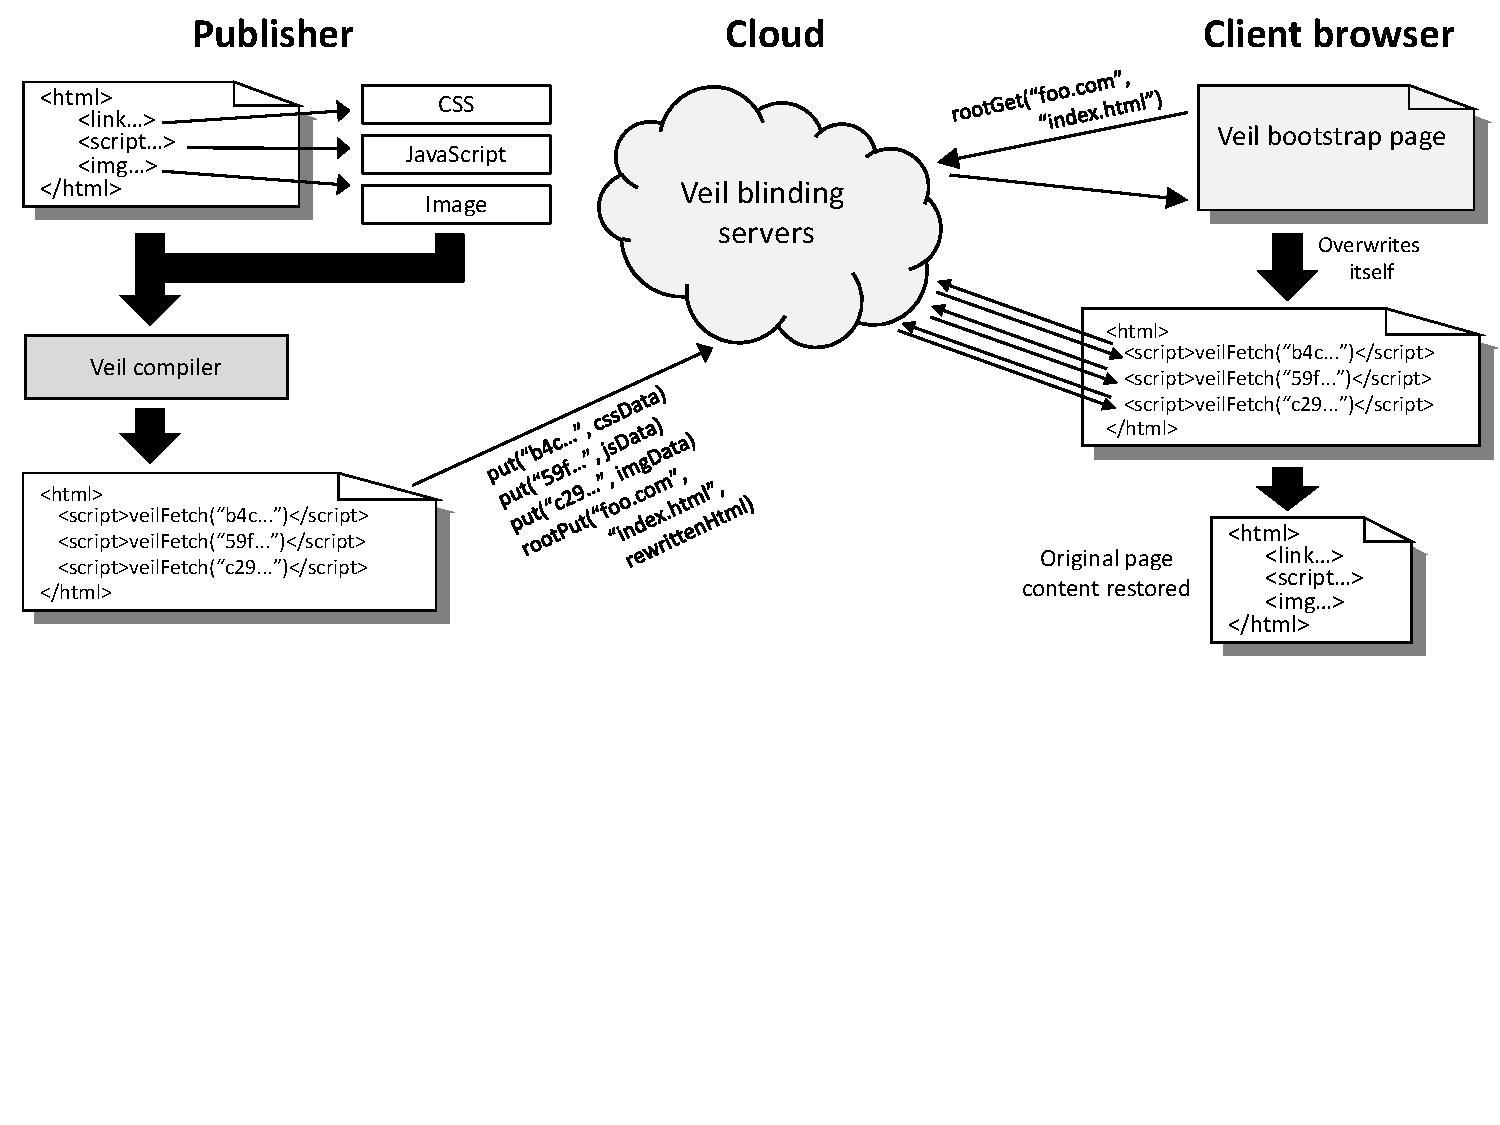
\includegraphics[width=\textwidth]{veil-figs/arch_small_cropped}
	\caption{The Veil architecture (cryptographic operations omitted for clarity).}
	\label{fig:arch}
\end{figure*}

As shown in Figure~\ref{fig:arch}, the Veil framework  %!!!jwm: Arg, the fig ref isn't resolving correctly.
consists of three components. The \emph{compiler}
transforms a normal web page into a new version
that implements static and dynamic privacy protections.
Web developers upload the compiler's output to
\emph{blinding servers}. These servers act as
intermediaries between content publishers and
content users, encrypting content. To load the Veil
page, a user first loads a small \emph{bootstrap page}.
The bootstrap asks for a per-user key and the
URL of the Veil page to load; the bootstrap then
downloads the appropriate objects from the blinding
servers and dynamically overwrites itself with
the privacy-preserving content in the target page.

In the remainder of this section, we describe Veil's
architecture in more detail. Our initial discussion
involves a simple, static web page that consists of
an HTML file, a CSS file, a JavaScript file, and an
image. We iteratively refine Veil's design to protect
against various kinds of privacy leakage. Then, we
describe how Veil handles more complex pages that
dynamically fetch and generate new content.


\subsubsection{The Veil Compiler and veilFetch()}
\label{sec:compiler}

The compiler processes the HTML in our example page (Figure~\ref{fig:arch}),
and finds references to three external objects (i.e.,
the CSS file, the JavaScript file, and the image).
The compiler computes a hash value for each object,
and then replaces the associated HTML tags with
dynamic JavaScript loaders for the objects. For
example, if the original image tag looked like this:
\begin{verbatim}
<img src="http://foo.com/img.jpg"/>
\end{verbatim}
the compiler would replace that tag with the following:
\begin{verbatim}
<script>veilFetch("b6a0d...");</script>
\end{verbatim}
where the argument to \texttt{veilFetch()} is the hash
name of the image. At page load time, when
\texttt{veilFetch()} runs, it uses an \texttt{XMLHttpRequest}
request to download the appropriate object from the
blinding service. In our example, the URL in the
\texttt{XMLHttpRequest} might be \texttt{http://veil.io/b6a0d...}.

Such a URL resides in the domain of the blinding
servers, not the domain of the original content
publisher. Furthermore, the URL identifies the underlying
object by hash, so the URL itself does not leak
information about the original publisher or the data
contained within the object. So, even though the
execution of \texttt{veilFetch()} may pollute
name-based interfaces like the DNS cache, a post-session
attacker which inspects those registries
cannot learn anything about the content that was fetched.
However, a network-observing attacker who sees a
\texttt{veilFetch()} URL can simply ask the blinding
server for the associated content, and then directly
inspect the data that the user accessed during the
private session!

To defend against such an attack, Veil associates
each user with a symmetric key $k_{user}$ (we describe
how this key is generated and stored in
Section~\ref{sec:bootstrap}). Veil also associates the
blinding service with a public/private keypair. When
\texttt{veilFetch(hashName)} executes, it does not
ask the blinding service for \texttt{hashName}---instead,
it asks for \texttt{<hashName>}$_{k_{user}}$. In the
HTTP header for the request, \texttt{veilFetch()} includes
$<k_{user}>_{PubKeyBServ}$, i.e., the user's symmetric
key encrypted by the blinding service's public key.
When the blinding service receives the request,
it uses its private key to decrypt $<k_{user}>_{PubKeyBServ}$.
Then, it uses $<k_{user}>$ to extract the hash
name of the requested object. The blinding service
locates the object, encrypts it with $k_{user}$,
and then sends the HTTP response back to the
client. Figure~\ref{fig:fetchProtocol} depicts
the full protocol.\footnote{%The protocol shown in
	%Figure~\ref{fig:fetchProtocol} requires a public
	%key operation for each request. However,
	A stateful blinding service can cache decrypted
	user keys and eliminate the public key operation
	from all but the user's first request.} In practice,
the blinding service's public/private
keypair can be the service's TLS keypair, as used
by HTTPS connections to the service. Thus, the
encryption of $k_{user}$ can be encrypted by the
standard TLS mechanisms used by an HTTPS connection.

Once \texttt{veilFetch()} receives the response,
it decrypts the data and then dynamically
reconstructs the appropriate object, replacing
the script tag that contained \texttt{veilFetch()}
with the reconstructed object. The compiler
represents each serialized object using JSON~\cite{json};
Figure~\ref{fig:imgJson} shows an example
of a serialized image. To reinflate
the image, \texttt{veilFetch()} extracts
metadata like the image's width and height,
and dynamically injects an image tag into
the page which has the appropriate attributes.
Then, \texttt{veilFetch()} extracts the
Base64-encoded image data from the JSON,
and sets the \texttt{src} attribute
of the image tag to a data URL~\cite{dataUrl}
which directly embeds the Base64 image
data. This causes the browser to load the
image. \texttt{veilFetch()} uses similar
techniques to reinflate other content types.

\begin{figure}
	\centering
	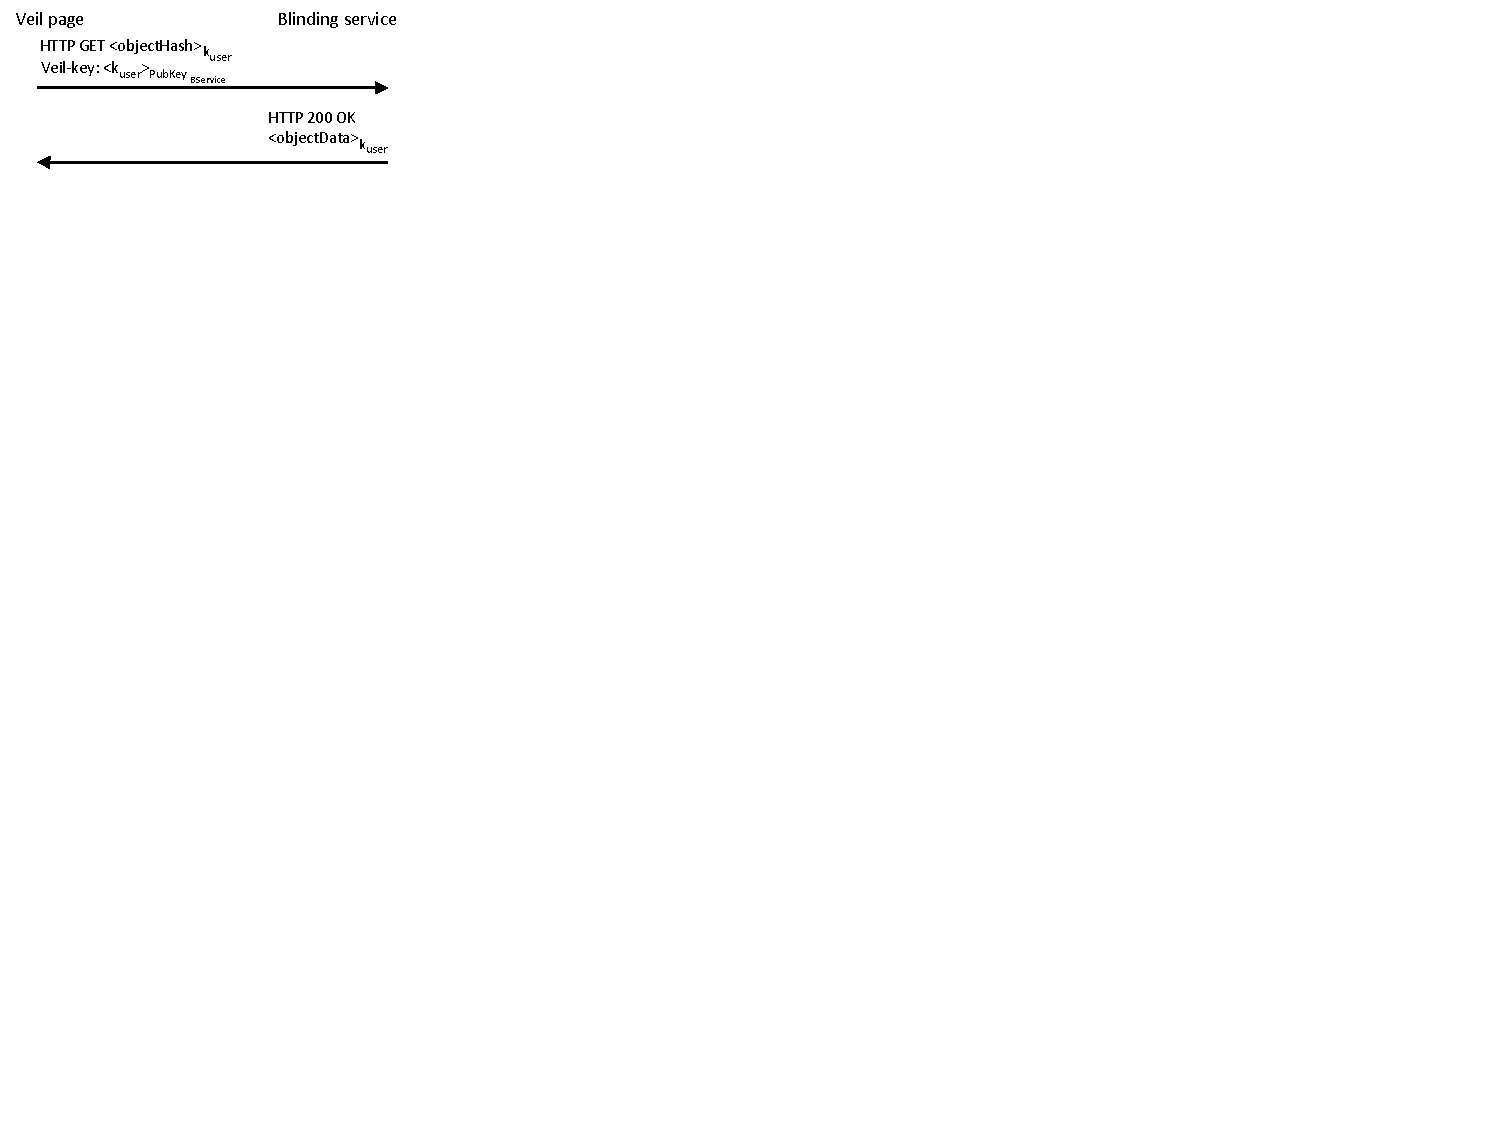
\includegraphics{veil-figs/fetchProtocol_cropped}
	\caption{The \texttt{veilFetch()} protocol.}
	\label{fig:fetchProtocol}
\end{figure}

\begin{center}
\begin{figure}
		\begin{BVerbatim}
		    {"img_type": "jpeg",
		    "dataURI": "ab52f...",
		    "tag_attrs": {"width": "20px",
		    "height": "50px"}}
		\end{BVerbatim}	
	\caption{A serialized \texttt{<img>} tag.}
	\label{fig:imgJson}
\end{figure}
\end{center}

This client-server protocol has several nice
properties. First, it solves the replay
problem---if an attacker wants to replay
old fetches, or guess visited URLs (as in a
CSS-based history attack~\cite{cssHistoryAttack,cssHistoryAttack2}),
the attacker will not be able to decrypt the
responses unless she has the user's key. Also,
since the blinding service returns encrypted
content, that encrypted content is what would
reside in the browser cache. Thus, Veil pages
can now persist data in the browser cache
such that only the user can decrypt and inspect
that content. Of course, a page does not have
to use the browser cache---when a publisher
uploads an object to the blinding service,
the publisher indicates the caching headers that the
service should return to clients.

In addition to uploading data objects like
images to the blinding service, the compiler
also uploads ``root'' objects. Root objects
are simply top-level HTML files like \texttt{foo.com/index.html}.
Root objects are signed with the publisher's
private key, and are stored in a separate
namespace from data objects using a 2-tuple
key that consists of the publisher name
(\texttt{foo.com}) and the HTML name
(\texttt{index.html}). Unlike data objects,
which are named by hash (and thus self-verifying),
root objects change over time as the associated
HTML evolves. Thus, root objects are
signed by the publisher to guarantee
authenticity and allow the blinding service
to reject fraudulent updates.


\subsubsection{The Blinding Service}
\label{sec:bservs}

In the previous section, we described the
high-level operation of the blinding service.
It exports a key/value interface to content
publishers, and an HTTP interface to browsers.
The HTTP code path does content encryption
as described above. As described in
Section~\ref{sec:mutation}, the blinding
service also performs \emph{content mutation}
to protect RAM artifacts that spill to disk;
mutation does not provide cryptographically
strong protections, but it does significantly
raise the difficulty of post-session forensics.
%We discuss specific mutation techniques in
%Section~\ref{sec:mutation}); for now, we note
%that mutation is a complement to heap walking
%(\S\ref{sec:heapWalk}), a separate technique
%which decreases the likelihood that RAM
%artifacts page out in the first place.
The blinding servers also implement the DOM
hiding protocol (\S\ref{sec:domHiding}), which
Veil sites can use to prevent exposing \emph{any}
site-specific HTML, CSS, or JavaScript to client
browsers.

%Content encryption allows Veil pages to
%securely persist state in the browser cache.
%However, this encryption cannot protect an
%application's in-memory data structures if those
%structures are reflected to disk, e.g., during
%paging, or when the system goes into hibernation
%mode and the OS takes a RAM snapshot. We assume
%that an attacker gains access to the user's machine
%after the private session has terminated, but
%operating systems frequently do not zero-out
%swap files and hibernation files. This allows
%forensic tools to find evidence of prior browsing
%sessions, \emph{even if those sessions used
%a native browser privacy mode}~\cite{aggarwal10,magnetForensicsChrome,ohana13}. 

%To make it more difficult for attackers to
%analyze memory artifacts, the blinding service
%\emph{mutates} the content that it returns to
%clients. Mutation generates objects that are
%structurally different from (but semantically
%%equivalent to) the canonical versions that
%were uploaded by the publisher. Content mutation
%ensures that, on different clients, each
%in-memory representation of an object is
%different. This prevents replay fingerprinting
%attacks in which the adversary loads a candidate
%private page on his own browser, extracts RAM
%artifacts, and then compares those artifacts
%to those that reside in the user's page file
%or hibernation file. As we describe below,
%mutation also makes it difficult for attackers
%to perform a first-principles analysis on memory
%images.

The blinding service can be implemented
in multiple ways, e.g., as a peer-to-peer
distributed hash table~\cite{pastry,chord},
a centralized service that is run by a
trusted authority like the EFF,
or even a single cloud VM that is paid for and
operated by a single privacy-conscious user. In
practice, we expect a blinding service to be run
by an altruistic organization like the EFF, or by
altruistic individuals (as in Tor~\cite{tor}),
or by a large set of privacy-preserving
sites who will collaboratively pay for the cloud
VMs that run the blinding servers. Throughout the
dissertation, we refer to a single blinding service
\texttt{veil.io} for convenience.
However, independent entities can simultaneously
run independent blinding services.

Veil's publisher-side protocol is compatible
with accounting, since the blinding service knows
which publisher uploaded each object, and how many
times that object has been downloaded by clients.
Thus, it is simple for a cloud-based blinding service
to implement proportional VM billing, or cost-per-download
billing. In contrast, an altruistic blinding service
(e.g., implemented atop a peer-to-peer DHT~\cite{pastry,chord})
could host anonymous object submissions for free.
%To minimize the client-perceived fetch latencies
%for blinded objects, the blinding servers should
%be widely distributed, similar to CDN nodes.

\subsubsection{The Same-origin Policy}
\label{sec:sop}

A single web page can aggregate content from a
variety of different origins. As currently
described, Veil maps all of these objects to
a single origin: at compile time, Veil downloads
the objects from their respective domains, and
at page load time, Veil serves all of the
objects from \texttt{https://veil.io}.

The browser uses the same-origin policy~\cite{sop}
to constrain the interactions between content
from different origins. Mapping all content to
a single origin would effectively disable
same-origin security checks. Thus, Veil's static
rewriter injects the \texttt{sandbox} attribute~\cite{iframeSandbox}
into all \texttt{<iframe>} tags. Using this
attribute, the rewriter forces the browser
to give each frame a unique origin with respect
to the same-origin policy. This means that,
even though all frames are served from the
\texttt{veil.io} domain, they cannot tamper
with each other's JavaScript state. In our current
implementation of the compiler, developers are
responsible for ensuring that dynamically-generated
frames are also tagged with the \texttt{sandbox}
attribute; however, using DOM virtualization~\cite{treehouse,mugshot},
the compiler could inject DOM interpositioning
code that automatically injects \texttt{sandbox}
attributes into dynamically-generated frames.

DOM storage~\cite{domStorage} exposes the
local disk to JavaScript code using a key/value
interface. DOM storage is partitioned by origin,
i.e., a frame can only access the DOM storage of
its own domain. By assigning an ephemeral, unique
origin to each frame, Veil seemingly prevents
an origin from reliably persisting data across
multiple user sessions of a Veil page. To solve
this problem, Veil uses indirection. When a
frame wants to access DOM storage, it first
creates a child frame which has the special URL
\texttt{https://veil.io/domStorage}. The child
frame provides Veil-mediated access to DOM storage,
accepting read and write requests from the parent
frame via \texttt{postMessage()}. Veil associates
a private storage area with a site's public key,
and engages in a challenge/response protocol
with a frame's content provider before agreeing
to handle the frame's IO requests; the challenge/response
traffic goes through the blinding servers (\S\ref{sec:dynamic}).
The Veil frame that manages DOM storage employs
the user's key to encrypt and
integrity-protect data before writing it,
ensuring that post-session attackers cannot
extract useful information from DOM storage
disk artifacts.

Since Veil assigns random, ephemeral origins
to frames, cookies do not work in the standard
way. To simulate persistent cookies, an origin
must read or write values in DOM storage. Sending
a cookie to a server also requires explicit
action. For example, a Veil page which contains
personalized content might use an initial piece
of non-personalized JavaScript to find the local
cookie and then generate a request for dynamic
content (\S\ref{sec:dynamic}).

\subsubsection{The Bootstrap Page}
\label{sec:bootstrap}
Before the user can visit any Veil sites, she
must perform a one-time initialization step
with the Veil bootstrap page (e.g., \texttt{https://veil.io}).
The bootstrap page generates a private symmetric key for
the user and places it in local DOM storage,
protecting it with a user-chosen password. Veil
protects the in-memory versions of the password and
symmetric key with heap walking (\S\ref{sec:heapWalk})
to prevent these cleartext secrets from paging to disk.

Later, the user determines the URL (e.g., \texttt{foo.com/index.html})
of a Veil site to load. The user should discover
this URL via an already-known Veil page like a
directory site, or via out-of-band mechanisms like a
traditional web search on a different machine than the
one needing protection against post-session attackers; looking
for Veil sites using a traditional search engine
on the target machine would pollute client-side state
with greppable content. Once the user possesses the
desired URL, she returns to the bootstrap page. The
bootstrap prompts the user for her password, extracts
her key from local storage, and decrypts it with the
password. The bootstrap then prompts the user for
the URL of the Veil page to visit. The bootstrap
fetches the root object for the page. Then, the
bootstrap overwrites itself with the HTML in the
root object. Remember that this HTML is the output
of the Veil compiler; thus, as the browser loads
the HTML, the page will use \texttt{veilFetch()}
to dynamically fetch and reinflate encrypted objects.

Once the bootstrap page overwrites itself, the user
will see the target page. However, no navigation will
have occurred, i.e., the browser's address bar will
still say \texttt{https://veil.io}. Thus,
the browser's history of visited pages will
never include the URL of a particular Veil page,
only the URL of the generic Veil bootstrap. The
compiler rewrites links within a page so that, if
the user clicks a link, the page will fetch the
relevant content via a blinded URL, and then deserialize
and evaluate that content as described above.

\subsubsection{Protecting RAM Artifacts}
\label{sec:heapWalk}

As a Veil page creates new JavaScript objects,
the browser transparently allocates physical
memory pages on behalf of the site. Later,
the OS may swap those pages to disk if memory
pressure is high and those pages are infrequently
used. JavaScript is a high-level, garbage-collected
language that does not expose raw memory addresses.
Thus, browsers do not define JavaScript interfaces
for pinning memory, and Veil has no explicit way
to prevent the OS from swapping sensitive data
to disk.

By frequently accessing sensitive JavaScript
objects, Veil \emph{can} ensure that the
underlying memory pages are less likely to be
selected by the OS's LRU replacement algorithm.
Veil's JavaScript runtime defines a \texttt{markAsSensitive(obj)}
method; using this method, an application indicates
that Veil should try to prevent \texttt{obj}
from paging to disk. Internally, Veil maintains
a list of all objects passed to \texttt{markAsSensitive()}.
A periodic timer walks this list, accessing every
property of each object using JavaScript reflection
interfaces. Optionally, \texttt{markAsSensitive()} can
recurse on each object property, and touch every
value in the object tree rooted by \texttt{obj}.
Such recursive traversals make it easier for
developers to mark large sets of objects at
once. JavaScript defines a special \texttt{window}
object that is an alias for the global namespace, so
if an application marks \texttt{window} as
recursively sensitive, Veil will periodically
traverse the entire heap graph that is reachable
from global variables. Using standard techniques
from garbage collection algorithms, Veil can
detect cycles in the graph and avoid infinite
loops.

\texttt{markAsSensitive()} maintains references
to all of the sensitive objects that it has ever
visited. This prevents the browser from garbage
collecting the memory and possibly reusing it
without applying secure deallocation~\cite{chow05}.
At page unload time, Veil walks the sensitive list
a final time, deleting all object properties.
Since JavaScript does not expose raw memory,
Veil cannot \texttt{memset()} the objects to
zero, but deleting the properties does make
it more difficult for a post-session attacker
to reconstruct object graphs.

Sensitive data can reside in the JavaScript
heap, but it can also reside in the memory
that belongs to the renderer. The renderer is
the browser component that parses HTML,
calculates the screen layout, and repaints
the visual display. For example, if a page
contains an HTML tag like \texttt{<b>Secret</b>},
the cleartext string \texttt{Secret} may
page out from the renderer's memory. As another
example, a rendered page's image content
may be sensitive.

The renderer is a C++ component that is
separate from the JavaScript engine;
JavaScript code has no way to directly
access renderer state. However, JavaScript
can indirectly touch renderer memory
through preexisting renderer interfaces.
For example, if the application creates
an empty, invisible \texttt{<img>} tag,
and injects the tag into the page's HTML,
the browser invalidates the page's layout.
If the application then reads the size
of the image tag's parent, the browser is
forced to recalculate the layout of the
parent tag. Recalculating the layout
touches renderer memory that is associated
with the parent tag (and possibly other
tags). Thus, Veil can walk the renderer
memory by periodically injecting invisible
tags throughout the HTML tree (forcing
a relayout) and then removing those
tags, restoring the original state of
the application.

The browser's network stack contains memory
buffers with potentially sensitive content
from the page. However, Veil only transmits
encrypted data over the network, so network
buffers reveal nothing to an attacker if
they page out to disk and are subsequently
recovered. Importantly, Veil performs
heap walking on the user's password and
symmetric key. This prevents those secrets
from paging out and allowing an attacker
to decrypt swapped out network buffers.

\subsubsection{Mutation Techniques}
\label{sec:mutation}
Veil's main protection mechanism for RAM
artifacts is heap walking, and we show in
Section~\ref{sec:privLeaks} that heap walking
is an effective defense during expected rates
of swapping. However, Veil provides a second
line of defense via content mutation. Mutation
ensures that, each time a client loads a page,
the page will return different HTML, CSS, and
JavaScript, even if the baseline version of the
page has not changed. Mutation makes grep-based
attacks more difficult, since the attacker
cannot simply navigate to a non-Veil version
of a page, extract identifying strings from the
page, and then grep local system state for those
strings. Content mutation is performed by the
blinding servers (\S\ref{sec:bservs}); below,
we briefly sketch some mutation techniques
that the blinding servers can employ.

Note that blinding servers can mutate content
in the background, \textit{before} the associated
pages are requested by a client. For example,
blinding servers can store a pool of mutated
versions for a single object, such that, when
a client fetches HTML that refers to the
object, the blinding server can late-bind
the mutated version that the page references.
Using this approach, mutation costs need not
be synchronous overheads that are paid when
a client requests a page. In addition, 
when a user requests a Veil page,
the blinding servers update the corresponding 
hashes for the mutated objects in the root object
before sending it to the user
to preserve the self-verification property of 
Veil objects described in Section~\ref{sec:compiler}. \\

\noindent
{\bf JavaScript:} To mutate JavaScript files, the
blinding service uses techniques that are adapted
from metamorphic viruses~\cite{hunting06}. Metamorphic
viruses attempt to elude malware scanners by
ensuring that each instantiation of the virus has
syntactically different code that preserves the
behavior of the base implementation. For example,
functions can be defined in different places, and
implemented using different sequences of assembler
instructions that result in the same output.

Our prototype blinding service mutates JavaScript code
using straightforward analogues of the transformations
described above. JavaScript code also has
a powerful advantage that assembly code
lacks---the \texttt{eval()} statement provides a
JavaScript program with the ability to emit new
mutated code at runtime. Such ``\texttt{eval()}-folding''
is difficult to analyze~\cite{zozzle}, particularly
if the attacker can only recover a partial set of
RAM artifacts for a page.\footnote{Some .NET viruses
	already leverage access to the runtime's reflection
	interface to dynamically emit code~\cite{szor05}.}

However, note that if a faulty blinding server forgets to mutate invocations
of \texttt{veilFetch(hashName)}, then unscrambled object
hash names may be paged out to disk in JavaScript source code! If an attacker
recovered such artifacts, he could directly replay the
object fetches that were made by the private session.
Thus, JavaScript mutation is a core responsibility for
the blinding service.\\

\noindent
{\bf HTML and CSS:} The grammars for HTML and CSS are
extremely complex and expressive. Thus, there are many
ways to represent a canonical piece of HTML or
CSS~\cite{webAppObfuscation}. For example, HTML allows %!!!Make sure I'm getting the details of this right.
a character to be encoded as a raw binary symbol in a
character encoding like \texttt{UTF-8} or \texttt{Unicode-16}.
HTML also allows characters to be expressed as escape
sequences known as HTML entities. An HTML entity consists
of the token ``\&\#'' followed by the Unicode code point
for a character and then a semicolon. For instance, the
HTML entity for ``a'' is ``\&\#97;''. The HTML
specification allows an HTML entity to have leading
zeroes which the browser ignores; the specification
also allows for code points to be expressed in
hexadecimal. Thus, to defeat simple exact-match
greps of HTML artifacts, the blinding service
can randomly replace native characters with random
HTML entity equivalents.

There are a variety of more sophisticated techniques
to obfuscate HTML and CSS. For a fuller exploration
of these topics, we defer the reader to other
work~\cite{webAppObfuscation}. Our blinding service
prototype uses random HTML entity mutation. It also
obscures the HTML structure of the page using
randomly inserted tags which do not affect the
user-perceived visual layout of the page.\\

\noindent
{\bf Images:} The blinding service can automatically
mutate images in several ways. For example, the
blinding service can select one of several formats
for a returned image (e.g., JPEG, PNG, GIF, etc.).
Each instantiation of the image can have a different
resolution, as well as different filters that are
applied to different parts of the visual spectrum.
Web developers can also use application-specific
knowledge to generate more aggressive mutations,
such as splitting a single base image into two
semi-transparent images that are stacked atop each
other by client-side JavaScript. %!!!Can you actually do this? :-)
As explained in our threat model (\S\ref{sec:threatModel}),
Veil does not protect against leaks of the raw
display bitmap that resides in GPU memory; thus,
the mutation techniques from above are sufficient
to thwart grep-based forensics on memory artifacts from
the DOM tree. For a more thorough discussion
of image mutation techniques that thwart
classification algorithms, we defer to literature
from the computer vision community~\cite{biggio11}.\\

% Orphan text that was removed from the intro.
% 
% To implement blinded references, Veil introduces a new
% set of \emph{blinding servers}. These servers sit between
% between users and application developers. Developers
% upload hash-named content to blinding servers, and users
% load a target page using Veil's bootstrap page, which
% gathers blinded objects via HTTP and uses them to
% dynamically reconstruct the target page. Blinding servers
% assist with mutating and encrypting content, but their
% clients can verify the integrity of blinded content
% using cryptography.
%
% From the perspective of a web browser, blinding servers
% export the standard HTTP interface and look like normal web
% servers. However, the blinding service can be implemented
% in multiple ways, e.g., as a distributed hash
% table~\cite{pastry,chord} or a centralized service run by
% a trusted authority. In practice, we expect that large
% groups of privacy-preserving sites will collaboratively
% pay for cloud VMs that run the blinding service
% (\S\ref{sec:bservs}). Blinding servers are compatible
% with per-publisher accounting mechanisms, so Veil can
% track how much traffic is associated with each Veil
% site and implement proportional VM billing.


% !!!Do we want to mention this?
% Metamorphic content and Veil strings also allow
% us to thwart forensics which looks at browser memory
% consumption to fingerprint pages~\cite{memento}.

\subsubsection{Dynamic Content}
\label{sec:dynamic}

At first glance, Veil's compile-time binding of
URLs to objects seems to prevent a publisher
from dynamically generating personalized user
content. However, Veil can support dynamic
content generation by using the blinding
service as a proxy that sits between the
end-user and the publisher. More specifically,
a Veil page can issue an HTTP request with
a \texttt{msg-type} of ``forward''. The body
of the request contains two things: user information
like a site-specific Veil cookie (\S\ref{sec:sop}),
and a publisher name (e.g., \texttt{foo.com}).
The page gives the request a random hash name,
since the page will not cache the response.
When the blinding service receives the request,
it forwards the message to the publisher's
dynamic content server. The publisher generates
the dynamic content from the provided user
information, and then sends the content to the
blinding service, who forwards it to the client
as the HTTP response to the client's ``forward''
request. The client and the publisher can encrypt
the user information and the personalized content
if the blinding service is not trusted with
user-specific data; in this scenario, the content provider's web server
is responsible for mutating objects before returning
them to the client. Regardless, the content provider
must compile dynamically-generated content (\S\ref{sec:compiler}
and \S\ref{sec:porting}).

Another option is to start with the same forwarding
protocol as above, but instead of having
the publisher compile and mutate the content, the 
publisher just sends the unmodified user-specific
content back to the blinding servers. Then, the blinding
servers compile and mutate the content before
returning it to the user. 

The question is which of the two options is better. 
More specifically, should the blinding servers
or the publishers perform compilation and mutation?
Ideally, the end host
would manipulate the dynamic content as it might
contain sensitive user information, which can be 
encrypted on host and thus hidden from the blinding servers.
However, the downside is that all end hosts have to 
adopt Veil. Having the proxy perform the manipulation
solves this problem, but this scenario would
require the proxy to handle a heavier computation workload.
The networking community
has examined these tradeoffs in a similar context, 
so we refer the reader to that specific research for a more in-depth
discussion~\cite{flywheel,polaris}.
The performance overhead is minimal because only the dynamic
portions of the site have to be compiled during the page load, 
and more detailed numbers are in Section~\ref{sec:macrobench}.

\subsubsection{DOM Hiding}
\label{sec:domHiding}

Heap walking reduces the likelihood that in-memory browser
state will swap to disk. Content mutation ensures that, if
state does swap out, then the state will not contain greppable
artifacts from a canonical version of the associated page.
However, some Veil sites will be uncomfortable with sending
\emph{any} site-specific HTML, CSS, or JavaScript to a client,
even if that content is mutated. For example, a site might
be concerned that a determined sysadmin can inspect swapped-out
fragments of mutated HTML, and try to reverse-engineer the
mutation by hand.

To support these kinds of sites, Veil provides a mode of
operation called DOM hiding. In DOM hiding mode, the user's
browser essentially acts as a thin client, with the full
version of the page loaded on a remote server that belongs
to the content provider. The user's browser employs a generic,
page-agnostic JavaScript library to forward GUI events to
the content provider through the blinding service; the content
provider's machine applies each GUI event to the server-side
page, and then returns an image that represents the new state
of the page.

The advantage of DOM hiding is that site-specific HTML, CSS,
and JavaScript is never pushed to the user's browser. The
disadvantage is that each GUI interaction now suffers from
a synchronous wide-area latency. For some Veil sites,
this trade-off will be acceptable. We characterize the
additional interactive latency in Section~\ref{sec:dhEval}.

\begin{figure}
	\centering
	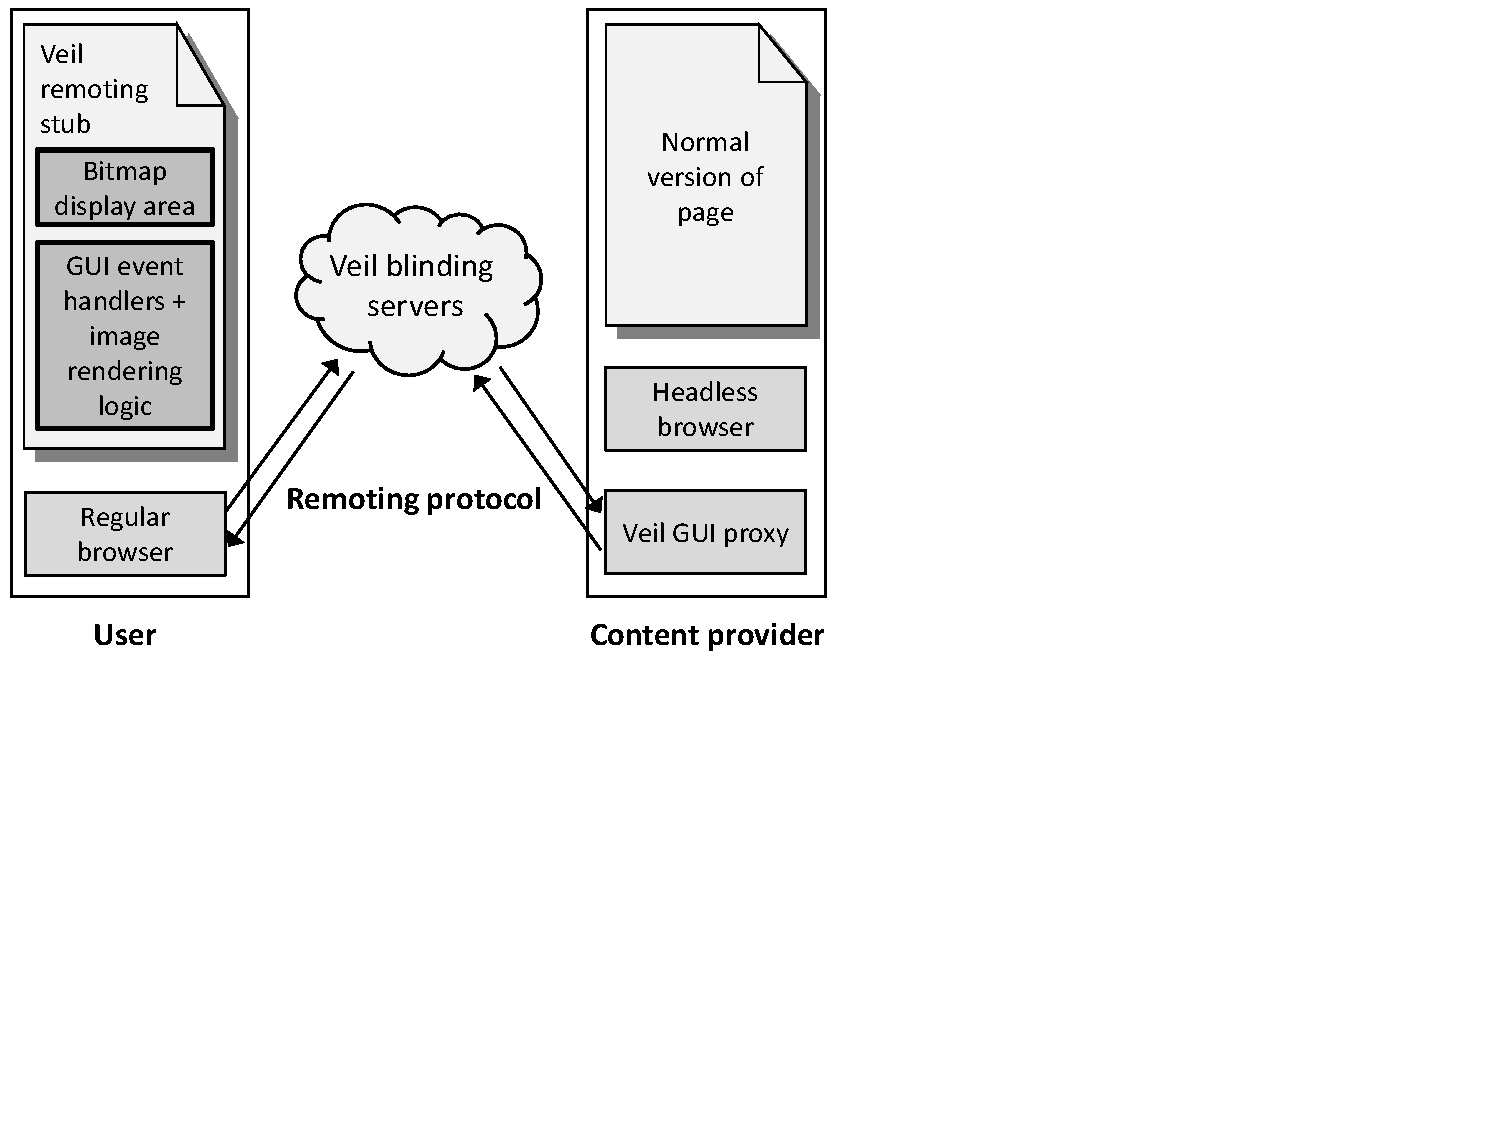
\includegraphics[width=\textwidth]{veil-figs/domHiding.pdf}
	\caption[Overview of DOM hiding mode]{With DOM hiding, the client-side remoting stub sends
		GUI events to the content provider, and receives bitmaps
		representing new page states. The page's raw HTML, CSS,
		and JavaScript are never exposed to the client.}
	\label{fig:domHiding}
\end{figure}

Figure~\ref{fig:domHiding} provides more details about how Veil
implements DOM hiding. The Veil bootstrap page receives the
URL to load from the user, as described in Section~\ref{sec:bootstrap}.
The bootstrap page then issues an initial HTTP request through
the blinding servers to the content provider.
The content provider returns a page-agnostic remoting stub;
this stub merely implements the client-side of the remote
GUI architecture. As the content provider returns the stub
to the user, the provider also launches a headless browser\footnote{A
	headless browser is one that does not have a GUI. However, a
	headless browser \emph{does} maintain the rest of the browser
	state; for example, DOM state can be queried using normal DOM
	methods, and modified through the generation of synthetic DOM
	events like mouse clicks.} like PhantomJS~\cite{phantomJS} to load
the normal (i.e., non-rewritten) version of the page. The
content provider associates the headless browser with a Veil
GUI proxy. The proxy uses native functionality in the headless
browser to take an initial screenshot of the page. The GUI
proxy then sends the initial screenshot via the blinding servers
to the user's remoting stub. The stub renders the image, and
uses page-agnostic JavaScript event handlers to detect
GUI interactions like mouse clicks and keyboard presses. 
The stub forwards those events to the GUI
proxy. The proxy replays those events in the headless
browser, and ships the resulting screen images back to the
client. Note that a page which uses DOM hiding will not
use encrypted client-side browser caching (\S\ref{sec:compiler})
or DOM storage (\S\ref{sec:sop})---there
will be no page-specific client-side state to store.

\subsubsection{Discussion}
\label{sec:discussion}

Veil tries to eliminate cleartext client-side
evidence of browsing activity. However, Veil does
not prevent the server-side of a web page from
tracking user information. Thus, Veil is compatible
with preexisting workflows for ad generation and
accounting (although advertising infrastructure
must be modified to use blinded URLs and
``forward'' messages).

% jwm: Hmm, on second read, this paragraph doesn't
%      seem very enlightening . . .
%
% Like all programs that perform cryptography, a Veil
% page is forced to store sensitive keys in cleartext
% form at certain points during execution. For example,
% the Veil page must load the cleartext user password into
% memory before it can decrypt the user's symmetric key;
% later, the page must use that cleartext symmetric key
% to decrypt objects that are returned by the blinding
% service. If an attacker can recover such material from
% a RAM artifact, it makes it easier to analyze other
% data that may have leaked from the private session
% (although content mutation will still present the
% attacker with challenges). The necessity for cleartext
% cryptographic keys is problematic, but it seems
% intrinsic to any program that performs cryptography.

If a Veil page wants to use the browser cache, Veil
employs encryption to prevent attackers from inspecting
or modifying cache objects. However, an attacker may
be able to fingerprint the site by observing the size
and number of its cached objects. Sun et al.~\cite{sun02} provide a
survey of techniques which prevent such fingerprinting attacks; 
their discussion is in the context of
protecting HTTPS sessions, but their defensive
techniques are equally applicable to Veil. The strongest
defense is to reduce the number of objects in a page.
Veil's compiler can easily do this by inlining objects
into HTML~\cite{silo}; for example, the compiler can
directly embed CSS content that the original HTML
incorporated via a link to an external file. The blinding
service can also inject noise into the distribution of object
sizes and counts. For example, when the service returns
objects to clients, it can pad data sizes to fixed offsets,
e.g., 2KB boundaries or power-of-2 boundaries. Alternatively,
the blinding service can map object sizes for page $X$ to
the distribution for object sizes in a different page
$Y$~\cite{wright09}. All of these defensive approaches
hurt performance in some way---inlining and merging
reduce object cacheability, and padding increases the
amount of data which must be encrypted and transmitted
over the network. Note that publishers must explicitly
enable client-side caching, so paranoid sites can simply
disable this feature.

%A private web service can inadvertently leak information
%about its user base via server-side timing channels
%~\cite{serverTimingAttacks}. For example, suppose that
%a service's login page requires a user to enter an
%email address. Further suppose that, on the web server,
%processing a login with a valid email address takes
%a different amount of time than processing a login
%that uses an invalid address. If an attacker knows a
%user's email address, he can reveal whether the user
%has visited the private site by navigating to the site
%himself, performing two login attempts (one with the
%user's real email address, and another with a fake
%email address), and observing whether the server-side
%timing is the same. Veil does not specifically address
%this attack, but Veil is compatible with solutions
%like the \texttt{mod\_timepad} Apache module~\cite{serverTimingAttacks}.

\subsection{Porting Legacy Applications}
\label{sec:porting}

In this section, we describe how Veil helps developers
to port legacy web pages to the Veil framework. In
particular, we provide case studies which demonstrate
how Veil's compiler and runtime library can identify
unblinded fetches and, in some cases, automatically
transform those fetches into blinded ones.\\

\noindent
{\bf Raw XMLHttpRequests:} Veil's compiler traverses
a statically defined HTML tree, converting raw URLs
into Veil hash pointers. However, a page's JavaScript
code can use \texttt{XMLHttpRequests} to dynamically
fetch new content. Veil's static HTML compiler does
not interpose on such fetches, so they will generate
unblinded transfers that pollute the client's DNS cache
and browser cache.

In debugging mode, Veil's client library shims the
JavaScript runtime~\cite{mugshot} and interposes on
the \texttt{XMLHttpRequest} interface. This allows
Veil to inspect the URLs in \texttt{XMLHttpRequests}
before the associated HTTP fetches are sent over the
network. Veil drops unblinded requests and writes the
associated URLs to a log. A web developer can then
examine this log and determine how to port the URLs.

For static content, one porting solution is to leverage
Veil's \textit{AJAX maps}. Once the debugging client
library has identified a page's raw \texttt{XMLHttpRequest}
URLs, the library sends those URLs to Veil's HTML
compiler. The compiler automatically fetches the associated
objects and uploads them to the object servers. Additionally,
when the compiler rewrites the HTML, it injects
JavaScript code at the beginning of the HTML which maps
the raw \texttt{XMLHttpRequest} URLs to the hash names
of the associated objects. Later, when the page is
executed by real users, Veil's shimmed \texttt{XMLHttpRequests}
use the AJAX map to convert raw URLs to blinded references.
Veil will drop requests that are not mentioned in
the translation map. This approach is complete from
the security perspective, since all unblinded \texttt{XMLHttpRequests}
will be dropped. However, for this approach to please users
(who do not want \textit{any} requests to drop),
Veil developers should use testing tools with good
coverage~\cite{monkeytest,clickmonkey,sahi} to ensure
that all of a page's \texttt{XMLHttpRequest} URLs are
mapped.

AJAX maps are unnecessary for native Veil pages
which always generate blinded \texttt{XMLHttpRequests}.
However, URL validation via \texttt{XMLHttpRequest}
shimming is useful when developers must deal with
complex legacy libraries.\\

\noindent
{\bf Dynamic tag generation:} A legacy page can generate
unblinded fetches by dynamically creating new DOM nodes
that contain raw URLs in \texttt{src} attributes. For
example, using \texttt{document.createElement()}, a page
can inject a new \texttt{<img>} tag into its HTML\@. A
page can also write to the \texttt{innerHTML} property
of a preexisting DOM node, creating a new HTML subtree
that is attached to the preexisting node. Neither type of
tag creation will be captured by \texttt{XMLHttpRequest}
shimming.

\texttt{XMLHttpRequest} shimming is a specific example
of a more general technique called DOM virtualization.
If desired, the entire DOM interface can be
virtualized~\cite{psj,treehouse,jigsaw}, allowing Veil to interpose
on all mechanisms for dynamic tag creation. However,
full DOM virtualization adds non-trivial performance
overhead---the native DOM implementation is provided by
the browser in fast C++ code, but a virtualized DOM is
implemented by the application in comparatively slow JavaScript
code. Furthermore, the full DOM interface is much more
complex than the narrow \texttt{XMLHttpRequest} interface. 

Our current implementation of Veil supports
\texttt{XMLHttpRequest} shimming, but not full DOM
virtualization. We leave the integration of Veil with
a full virtualization system~\cite{treehouseGit} as
future work.\\

\noindent
{\bf Unblinded links in CSS:} CSS files can directly
reference image objects using the \texttt{url()}
statement, e.g., \texttt{body\{background: url(`x.jpg')\}}.
After the Veil compiler processes HTML files, it
examines the associated CSS files and replaces raw
image links with inline data URLs. Thus, when the
Veil page loads a post-processed CSS file, the image
data will be contained within the CSS itself, and will
not require network fetches.\\

\noindent
{\bf Angular.js:} Angular~\cite{angular} is a popular
JavaScript framework that provides model-view-controller
semantics for web applications. Angular uses a
declarative model to express data bindings. For
example, the \texttt{\{\{\}\}} operator is used to embed
live views of the controller into HTML\@. The HTML
snippet \texttt{<img src=\{\{controller.x\}\}/>} instructs
Angular to dynamically update the content of the
\texttt{<img>} whenever the JavaScript value
\texttt{controller.x} changes. Many other popular
frameworks define a similar templating mechanism~\cite{backbone,kendo,ember}.

The \texttt{\{\{\}\}} operator is not part of the official
HTML grammar. To implement \texttt{\{\{\}\}} and other
kinds of data binding, Angular uses a dynamic DOM
node compiler. This compiler is a JavaScript file
that runs at the end of the page load, when the initial DOM
tree has been assembled. The compiler locates special
Angular directives like \texttt{\{\{\}\}}, and replaces
them with new JavaScript code and DOM nodes
that implement the data binding protocol.

Angular allows URLs to contain embedded \texttt{\{\{\}\}}
expressions. Since these URLs are not resolved until
runtime, Veil's static compiler cannot directly
replace those URLs with blinded ones. However, Veil
can rewrite Angular directives in a way that passes
control to Veil code whenever a data binding changes.
In the previous \texttt{<img>} example, Veil rewrites
the tag as follows:

\begin{verbatim}
<img src="0" alt={{controller.x}}/>
\end{verbatim}
The \texttt{src} attribute of the image is set to
a network path which is known to be nonexistent
(but whose URL does not leak private information).
When the page tries to load the image, the load
failure will invoke a custom \texttt{onerror}
handler that Veil has attached to the \texttt{window}
object. That handler will read the value of the
\texttt{alt} attribute, which will contain the
dynamic value of \texttt{controller.x}. Veil
will then issue a blinded fetch for the associated
image. In parallel, Veil also sets an Angular
\texttt{\$watch()} statement to detect future
changes in \texttt{\{\{controller.x\}\}}; when a
change occurs, Veil reads the new value, and then
blindly fetches and updates the image as before.
This basic approach is compatible with the template
semantics of other popular JavaScript
frameworks~\cite{backbone,kendo,ember}.

If dynamic Angular URLs can be drawn from an arbitrarily
large set, Veil uses the ``forward'' message type
from Section~\ref{sec:discussion} to bind the
raw URL to a blinded one. If the URL is drawn
from a finite set, the compiler can upload the
associated objects to the blinding service,
and then inject the page with a blinding
map that translates resolved Angular URLs
to the associated hash names. The blinding
service mutates that table in the same way
that it mutates the hash names passed to
\texttt{veilFetch()}.

\subsection{Implementation}
\label{sec:impl}

Our Veil prototype consists of a compiler,
a blinding server, a GUI proxy, a bootstrap page,
and a client-side JavaScript library that
implements \texttt{veilFetch{}()}
%, the \texttt{v\_str} object,
and other parts of the Veil runtime.

We implemented the compiler and the blinding
server in Python. The compiler uses
BeautifulSoup~\cite{beautifulSoup} to
parse and mutate HTML; the compiler also
uses the Esprima/Escodegen tool chain~\cite{esprima,escodegen}
to transform JavaScript code into ASTs, and
to transform the mutated ASTs back into
JavaScript. To implement cryptography, we use the
PyCrypto library~\cite{pyCrypto}
in the blinding server, and the native
Chrome WebCrypto API~\cite{webCrypto} 
in the Veil JavaScript library. We 
use OpenCV~\cite{opencv} to perform
image mutation on the blinding server.

To implement DOM hiding, we used Chrome 
running in headless mode as the browser
used by the content provider's GUI proxy.
The GUI proxy was written in Python, and
used Selenium~\cite{selenium} to take
screenshots and generate synthetic GUI
events within the headless browser.

\subsection{Evaluation}
\label{sec:eval}

In this section, we evaluate Veil's raw
performance, and its ability to safeguard
user privacy. Using forensic tools and
manual analysis, we find that blinded
references and encrypted objects are
sufficient to prevent information leakage
through the browser cache and name-based
interfaces like the DNS cache. We show
that Veil's heap walking techniques are
effective at preventing secrets from paging
out unless system-wide memory pressure is
very high. We also demonstrate that the performance
of our Veil's prototype is acceptable, with
page load slowdowns of 1.2x--3.25x.

\begin{figure*}
	\centering
	\begin{tabular}{lr}
		\toprule
		\bf Operation & \bf Speed \\
		\midrule
		Generate an AES key and encrypt it with RSA public key (2048 bit)  & 0.75 ms \\
		% Throughtput for verifying 2048 bit RSA PKCS 1 signature on index file & 215 MB/s \\
		Encrypt 64 character hash (blinded reference) & 0.16 ms \\
		Throughput for decryption using AES-CTR & 520 MB/s \\
		Throughput for verifying SHA256 hash of file & 220 MB/s \\
		\bottomrule
	\end{tabular}
	\caption{Overhead for client-side JavaScript cryptography using the WebCrypto API~\cite{webCrypto}.}
	\label{fig:cryptoCost}
\end{figure*}

All performance tests ran on a machine with
a 2 GHz Intel Core i7 CPU with 8GB of RAM.
Unless otherwise specified, those tests ran in
the Chrome browser, and we ran each experiment
100 times and measured the average. We configured
Veil to use 2048-bit RSA and 128-bit AES in CTR
mode. The phrase ``standard Veil mode''
corresponds to non-DOM hiding mode.

\subsubsection{Performance Microbenchmarks}
\label{sec:microbench}

Veil uses cryptography to implement blind references
and protect the data that it places in client-side storage.
Figure~\ref{fig:cryptoCost} depicts the costs %!!!jwm: For some reason, doing a ~\ref{fig:cryptoCost} doesn't work!
for those operations. Before a user can load a Veil
page, she must generate an AES key and encrypt it
with the blinding service's RSA key. This one time
cost is 0.75 ms. The remaining three rows in Figure~\ref{fig:cryptoCost}
depict cryptographic %!!!jwm: For some reason, doing a ~\ref{fig:cryptoCost} doesn't work!
overheads that Veil incurs during a page load.
\begin{itemize}
	%    \item After the bootstrap page downloads a
	%          top-level HTML file, the bootstrapper
	%          must verify that the file is signed by
	%          the publisher. This operation proceeds
	%          at 215 MB/s; so, for an 100 KB HTML file,
	%          Veil would require 0.5 ms to validate
	%          the signature.
	\item For \texttt{veilFetch()} to generate a
	blinded reference, it must encrypt a
	hash value with the user's AES key. This
	operation took 0.16 ms.
	\item When \texttt{veilFetch()} receives a
	response, it must decrypt that response
	with the AES key. That operation proceeds
	at 520 MB/s. For example, decrypting a
	300 KB image would require 0.6 ms.
	\item \texttt{veilFetch()} also validates the
	hash of the downloaded object. This
	proceeds at 220 MB/s, requiring 1.3 ms
	for a 300 KB image.
\end{itemize}
Figure~\ref{fig:cryptoCostServer} depicts the
cryptography overheads on the server-side of
the protocol. End-to-end, fetching a 300 KB
object incurs roughly 10 ms of cryptographic
overhead. 

\begin{figure}
	\centering
	\begin{tabular}{lr}
		\toprule
		\bf Operation & \bf Speed \\
		\midrule
		Decrypt AES key (2048 bit RSA)  & \phantom{0}3.1 ms \\
		Decrypt 64 char hash (blinded reference) & 0.04 ms \\
		Throughput for encryption using AES-CTR & 62 MB/s \\
		\bottomrule
	\end{tabular}
	\caption{Overhead for server-side operations using PyCrypto~\cite{pyCrypto}.}
	\label{fig:cryptoCostServer}
\end{figure}

\subsubsection{Performance Macrobenchmarks: Standard Veil Mode}
\label{sec:macrobench}

To measure the increase in page load
time that Veil imposes, we ported six sites
to the Veil framework.  \textbf{Washington Post}
is the biggest site that we ported, and contains
large amounts of text, images, and JavaScript
files. \textbf{Imgur} is a popular image-sharing
site; compared to the other test sites, it has
many images but less text. \textbf{Woot!} is an
e-commerce site that has a large amount of text
and images, but comparatively few scripts.
\textbf{Piechopper} is a highly dynamic site that
uses Angular (\S\ref{sec:porting}). Piechopper is
script-and-text heavy, but has few images.
\textbf{University} represents a university's
website. This site is the smallest
one that we tested, although it uses CSS with raw
URLs that Veil must blind (\S\ref{sec:porting}).
\textbf{Google} represents the results page for
the search term ``javascript.''  Most of that page's
JavaScript and CSS objects are inlined into
the HTML, meaning that they do not require
network fetches. 

To port a preexisting site to Veil, we had the
compiler download the top-level HTML file and
extract the URLs which referenced external objects like
images. The compiler downloaded those objects from
the relevant servers. After calculating hashes
for those objects (and converting raw URLs into
blinded ones), the compiler uploaded the objects
to the blinding server. Since preexisting sites
were not designed with Veil in mind, they
occasionally fetched content dynamically, e.g.,
via unblinded \texttt{<img>} tags generated by
JavaScript at runtime. For sites like this, we
observed which objects were dynamically fetched,
and then manually handed them to the compiler
for processing; we also manually rewrote the
object fetch code to refer to the compiler-generated
object names. Native Veil pages would invoke
the Veil runtime library to dynamically fetch
such content, avoiding the need for manual
rewriting. \\

\begin{figure}
	\centering
	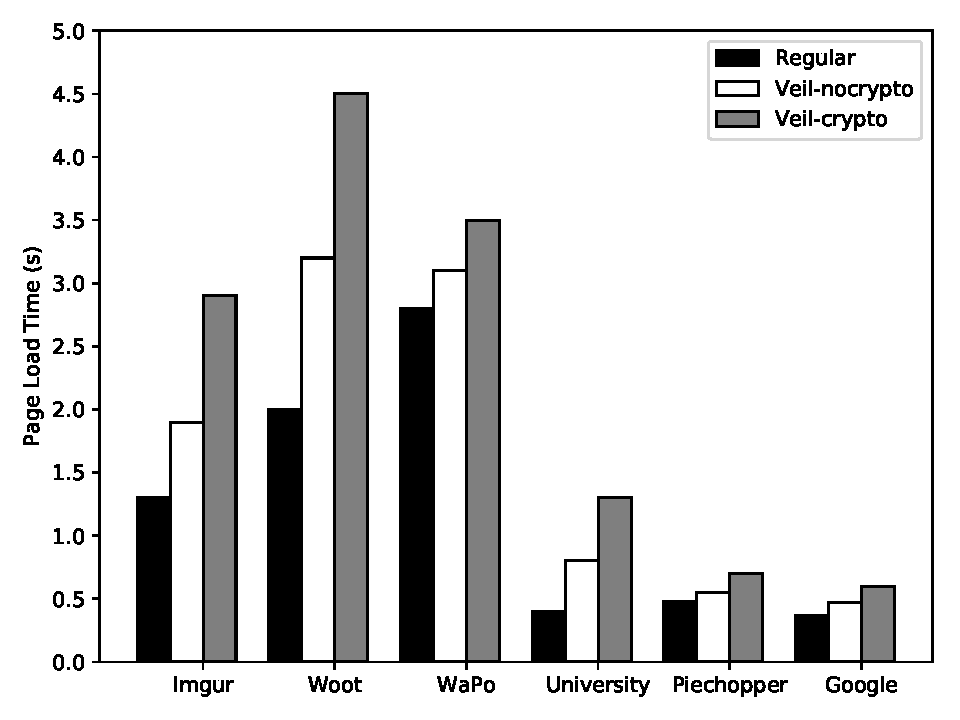
\includegraphics[width=\textwidth]{veil-figs/perf_graph.pdf}
	\caption{Page load times for each website: regular; with Veil (but no cryptography); with Veil (and using cryptography).}
	\label{fig:loadTime}
\end{figure}

\noindent
\textbf{Page load time:}
Figure~\ref{fig:loadTime} depicts the load times
for three versions of each site: the regular version
of the site, a Veil port that does not perform
cryptography, and a Veil port with cryptography
enabled. The regular versions of a page were loaded
from a localhost webserver, whereas the Veil pages
were loaded from a localhost blinding server. This setup
isolated the overhead of cryptography and content
mutation.

As shown in Figure~\ref{fig:loadTime}, page loads using Veil with
no cryptography were 1.25x--2x slower. This is mostly
due to extra computational overhead on the client.
For example, parsing overheads increased because,
as we quantify below, mutated objects were larger than
the baseline objects; for images, the browser also
had to Base64-decode the bitmaps before displaying
them.
%jwm: The below is no longer true, since we've
%     made the jump to asynchronous WebCrypto.
%Also note that \texttt{veilFetch()} downloads
%content synchronously, and that script tags
%halt the parsing process; since Veil replaces
%all image and CSS tags with script tags, this
%limits the browser's ability to continue parsing
%while previously visited tags are loading their
%content.
Veil with cryptography added another slowdown factor
of 1.1x--1.63x, with higher penalties for pages
with many objects (regardless of their type). The
end-to-end slowdown for the full Veil system
was 1.25x--3.25x. Note that these slowdowns were for
browsers with cold caches; 
Veil's overhead would
decrease with caching, since server-side
cryptography could be avoided. Also note that
the University site was a challenging case for
Veil, because the site was small in absolute size,
but has many small images. Thus,
Veil's per-blinded-reference cryptographic
overheads (see Figures~\ref{fig:cryptoCost} and~\ref{fig:cryptoCostServer}) %!!!jwm: See above re: broken fig command.
were paid more frequently. A Veil-optimized
version of the site would use image spriting~\cite{spriting}
to combine multiple small images into a single,
larger one.\\

\noindent
\textbf{Dynamic content overhead:}
As described in Section~\ref{sec:dynamic},
dynamic content has some overhead because it
has to be compiled during the page load.
Fortunately, the compilation cost for a single dynamic object
is typically small. For example, compiling a
100 KB image requires Base64-encoding it and
generating a few metadata fields, taking roughly
75 ms. Content providers or blinding servers 
can compile multiple dynamic objects in parallel. \\

\begin{figure}
	\centering
	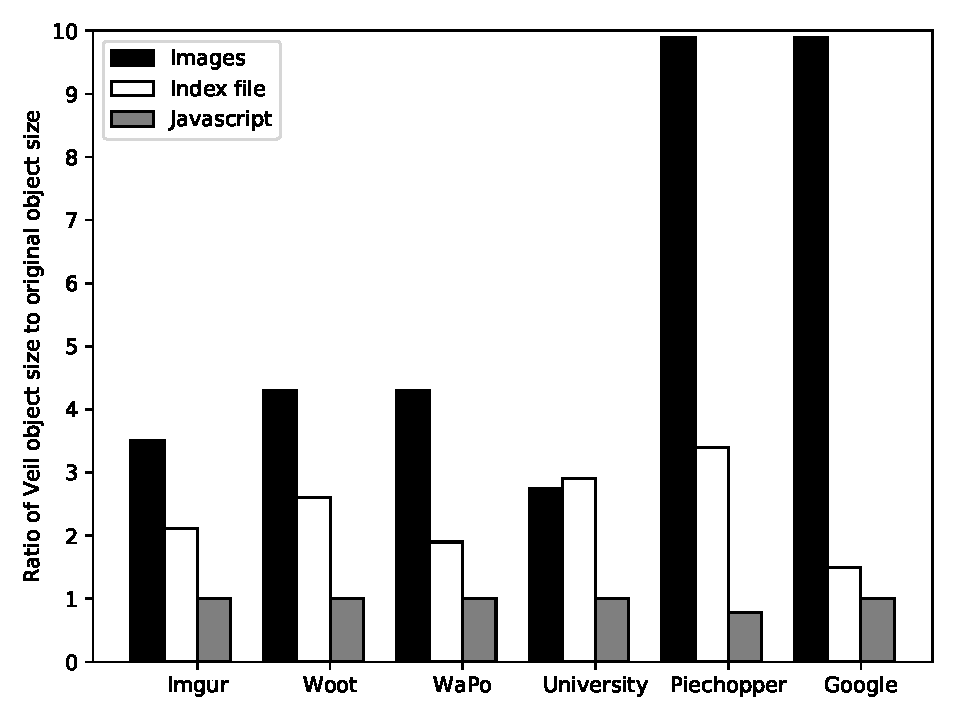
\includegraphics[width=\textwidth]{veil-figs/size_graph.pdf}
	\caption{Size increases for Veil's mutated objects.}
	\label{fig:mutateSize}
\end{figure}

\noindent
\textbf{Object growth:}
Figure~\ref{fig:mutateSize} shows how object sizes grew
after post-processing by Veil. Images experienced
two sources of size expansion: mutation and Base64
encoding. Base64 encoding resulted in a 1.33x size
increase. Our Veil prototype implements mutation via
the addition of Gaussian noise, with the resulting
size increases dependent on the image format. PNG
is lossless, so the addition of noise generated
a 10x size increase. In contrast, JPG is a lossy
format, so noise injection resulted in less than
a 2x size increase. The Piechopper and Google pages
contained many PNGs, and thus suffered from worse
image expansion than the other test pages.

As shown in Figure~\ref{fig:mutateSize}, mutated
JavaScript files typically remained the same size,
or became somewhat smaller---mutation adds source
code, but Veil passes the mutated code through
a minifier which removes extraneous whitespace
and rewrites variable names to be shorter. HTML
suffered from larger size increases, because
mutation tricks like random HTML entity encoding
strictly increase the number of characters in the
HTML. \\

\begin{figure}
	\centering
	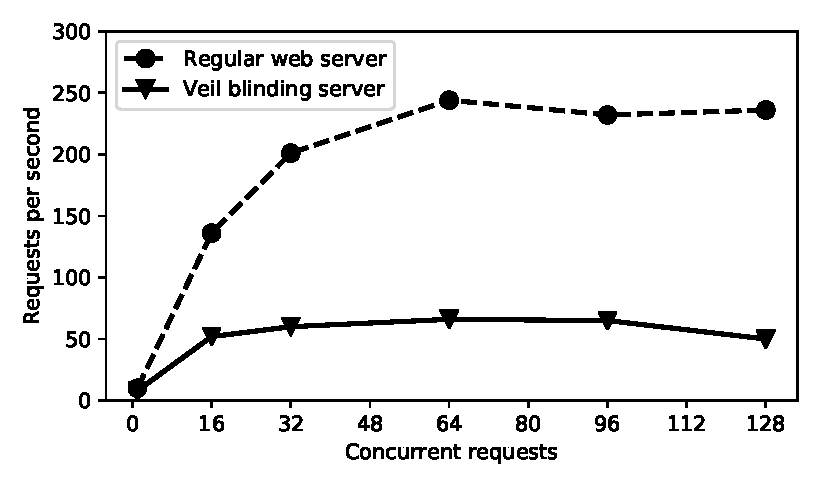
\includegraphics[width=\textwidth]{veil-figs/scalability_mit.pdf}
	\caption{Scalability comparison between a blinding server
		and a regular web server.}
	\label{fig:scalability}
\end{figure}

\noindent
\textbf{Server-side scalability:}
Figure~\ref{fig:scalability} shows the HTTP-level
request throughput of a Veil blinding server,
compared to the baseline performance of a blinding
server that performed none of Veil's added functionality
(and thus acted as a normal web server).
% The client and the servers were on the same machine, but
% client/server traffic used an emulated link
% with 25 ms latency and 500 Mbit/s of download
% bandwidth, to roughly simulate the public-facing
% network connection available to a blinding server
% run on an EC2 \texttt{c4.large} VM~\cite{!!!}. %  https://cloudspectator.com/wp-content/uploads/report/iaas_generational_aws_c3_c4.compressed.pdf
% Network emulation was performed using PF and dummynet.
HTTP requests were generated using \texttt{ab}, the Apache
benchmarking tool~\cite{ab}.

As shown in Figure~\ref{fig:scalability}, Veil
reduces web server throughput by roughly 70\%
due to the additional cryptographic operations
that Veil must perform. By quantifying 
Veil's scalability penalty for a fixed client load
compared to a regular web
server, blinding server hosts 
can know the additional servers needed 
to handle a specific load on a Veil page.
Remember that when
Veil operates in regular (i.e., non-DOM hiding
mode), Veil blinding servers mutate content in
the background, out of the critical path for an
HTTP response; thus, the slowdowns in Figure~\ref{fig:scalability}
are solely caused by synchronous cryptographic
operations. \\

\subsubsection{Preventing Information Leakage}
\label{sec:privLeaks}


{\bf Name-based interfaces:} To determine
how well Veil protects user privacy, we created
a baseline VM image which ran Lubuntu 13.10 and
had two different browsers (Firefox and Chrome). In
the baseline image, the browsers were installed, but they had
not been used to visit any web pages. We then ran
a series of experiments in which we loaded the
baseline image, opened a browser, and then visited
a single site. We took a snapshot of the browser's
memory image using \texttt{gcore}, and we also
examined disk state such as the browser
cache and the log entries for DNS resolution
requests. We did this for the regular and
Veil-enabled versions of each page described in
Section~\ref{sec:macrobench}.

In all tests, the Veil pages were configured to
store data in the browser cache, and in all tests,
the cache only contained encrypted data at the
end of the private session. Greps through the
memory snapshots and DNS records did not reveal
cleartext URLs or hostnames. Unsurprisingly,
the regular versions of the web pages left
unencrypted data in the browser cache, and
various cleartext URLs in name-based data
stores. To cross-validate these results, we
repeated these experiments on Windows, and used
the Mandiant Redline forensics tool~\cite{mandiant}
to search for post-session artifacts in persistent
storage. Redline confirmed that the only
cleartext URL in the browser history was the
URL for the Veil bootstrap page, and that all
other URLs were blinded.
%jwm: Maybe restore for camera-ready? Or not.
% Note that visiting a Veil page does not add
% a new entry to the browser's ``visited pages''
% history, because the bootstrap page overwrites
% itself without changing the URL in the address bar.
\\

\begin{figure}
	\centering
	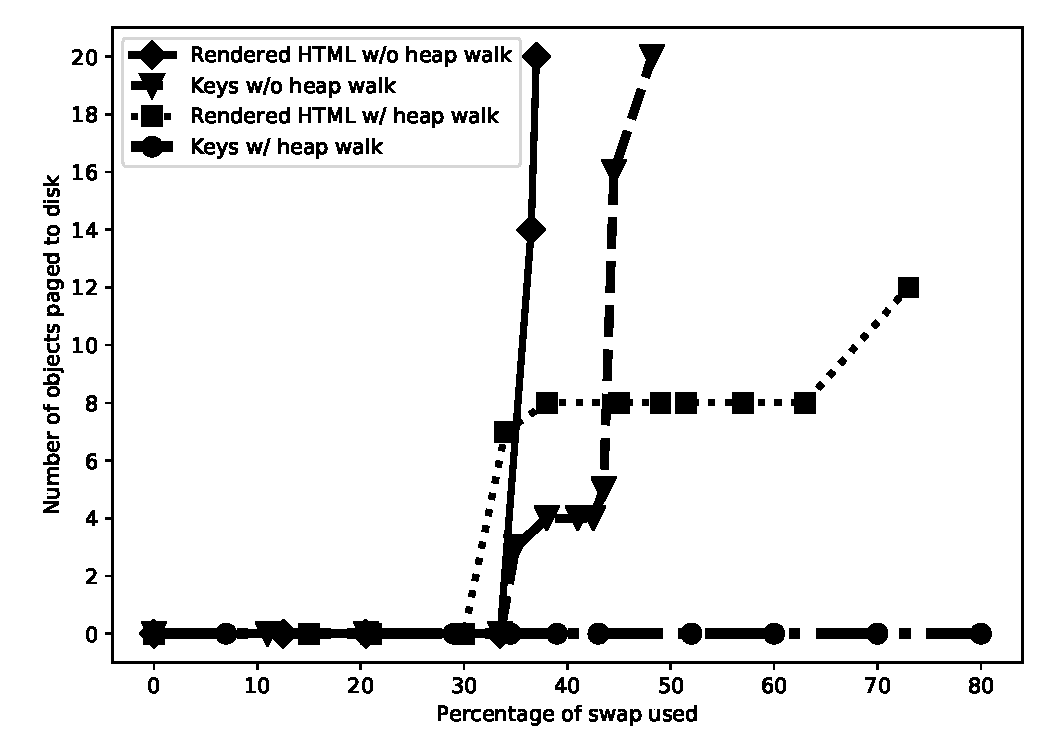
\includegraphics[width=\textwidth]{veil-figs/heapwalk_graph.pdf}
	\caption{The effectiveness of heap walking to prevent secrets from paging out.}
	\label{fig:heapWalking}
\end{figure}

\noindent
{\bf Protecting RAM artifacts:} To determine
whether heap walking can prevent secrets from
paging out, we wrote a C program which gradually
increases its memory pressure. The program allocates
memory without deallocating any, and periodically,
it reads the first byte in every allocated page
to ensure that the OS considers the page to be hot.
We ran the program inside of a QEMU VM with 1 GB
of swap space and 1 GB of RAM. We also ran a browser
inside of the VM. The browser had 20 open tabs.
Each tab had a Uint8Array representing a tab-specific
AES key, and a tab-specific set of strings in its
HTML. The control experiments did not do heap walking.
The test experiments used Veil's heap walking code
to touch the AES key and the renderer state.

The VM used the \texttt{pwritev} system call to
write memory pages to the swap file. To determine
whether secrets paged out as memory pressure
increased, we used strace to log the \texttt{pwritev}
calls. Since each tab contained a set of 
unique byte patterns, we could grep through our
\texttt{pwritev} logs to determine whether secret
RAM artifacts hit the swap file. We ran experiments
for increasing levels of memory pressure until the
VM became unresponsive, at roughly 75\% in-use
swap space.

Figure~\ref{fig:heapWalking} shows the results.
The x-axis varies the memory pressure, and the
y-axis depicts the number of tabs which suffered
data leakage, as determined by greps through the
\texttt{pwritev} log. Heap walking successfully
kept all of the secret keys from paging out, up
to the maximum 75\% of in-use swap space. Without
heap walking, keys begin to page out at 35\%
swap utilization; by 50\%, all keys had swapped
out. Note that the data points do not perfectly
align on the x-axis due to nondeterminism in
when the VM decides to swap data out.

Heap walking was less effective for renderer
memory pages. Those pages swapped out earlier
and immediately in the control case, around
35\% swap utilization. With Veil, renderer state
also began to leak at 35\% utilization, but
Veil still managed to safeguard 12 out of 20 tabs
up to 63\% swap utilization.

% Taking a memory snapshot using VMWare Workstation:
%  \begin{smitemize}
%    \item Load the VM, run a browser, interact with it,
%          then suspend it.
%    \item Use the \texttt{vmss2core} tool to create a
%          core dump. For example: \begin{verbatim}"C:\Program Files (x86)\VMware\VMware Player"\vmss2core Lubuntu-e49257cd.vmss Lubuntu-e49257cd.vmem\end{verbatim}
%    \item The core will be in a file named \texttt{vmss.core0}.
%  \end{smitemize}

% Generating a core dump for a Linux process:
%  \begin{smitemize}
%    \item Get the pid of the process.
%    \item sudo gcore -o XXX.core pid
%    \item strings -e l -a -t x XXX.core | grep YYY
%  \end{smitemize}

\subsubsection{DOM Hiding}
\label{sec:dhEval}

When Veil runs in DOM hiding mode, the client-side page
contains no site-specific, greppable content. Thus,
Veil does not need to perform heap walking (although
Veil does use blinding servers to eliminate information
leakage through name-based system interfaces). We loaded
our test pages in DOM hiding mode, and confirmed the absence
of site-specific content by grepping through VM images as
we did in Section~\ref{sec:privLeaks}. 

\begin{figure}
	\centering
	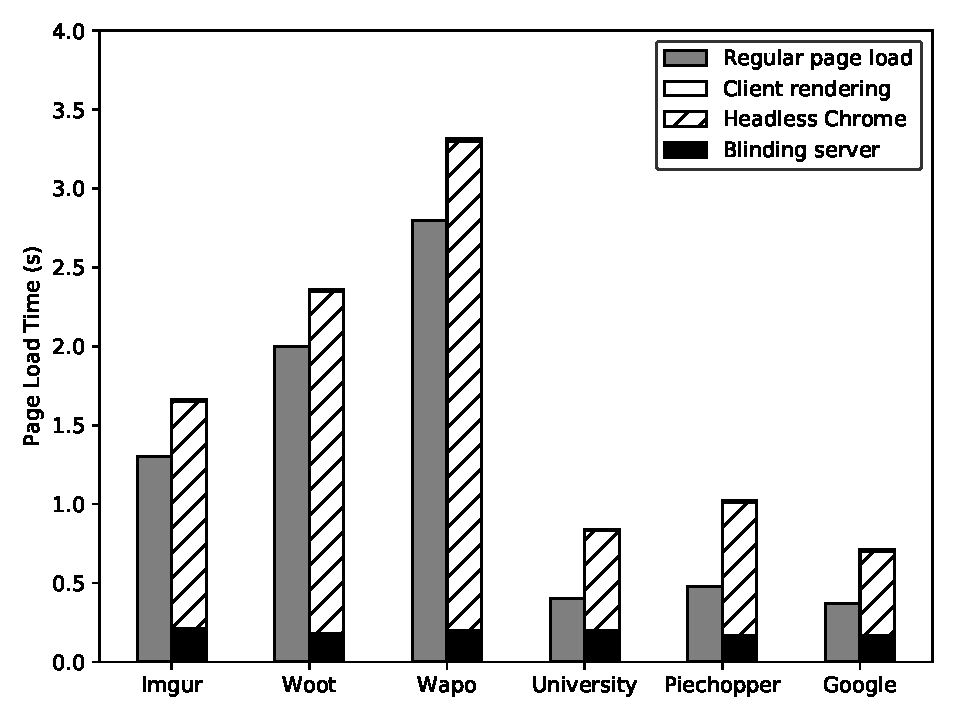
\includegraphics[width=\textwidth]{veil-figs/domhiding_loadtime.pdf}
	\caption{DOM hiding's impact on page load times.}
	\label{fig:dhPageLoad}
\end{figure}

\begin{figure}
	\centering
	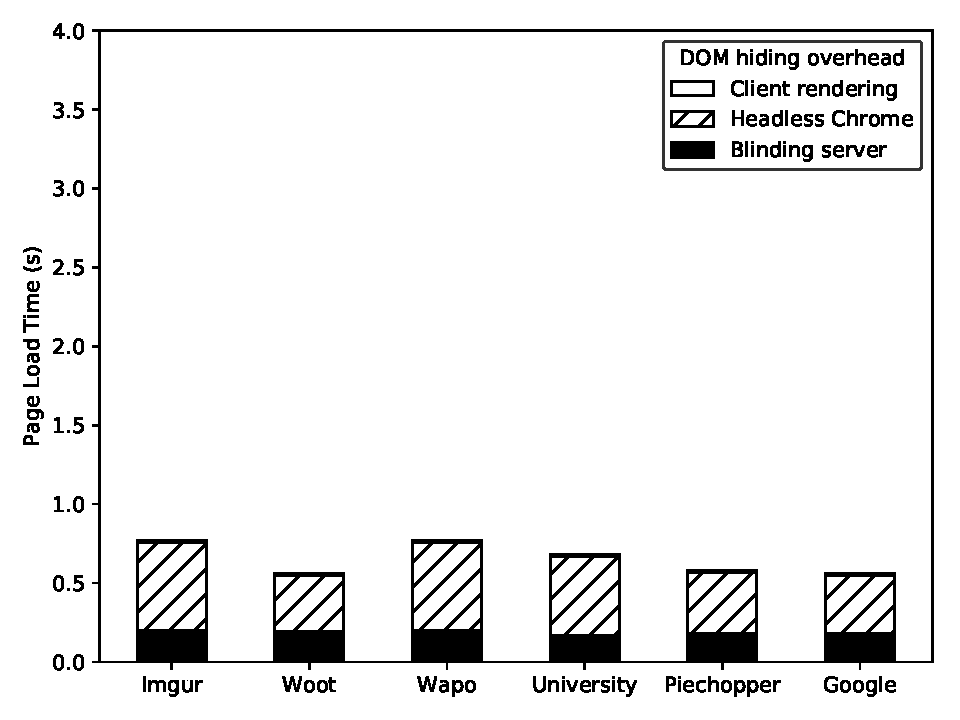
\includegraphics[width=\textwidth]{veil-figs/domhiding_click.pdf}
	\caption{The time that a DOM-hiding page needs to respond to a
		mouse click event.}
	\label{fig:dhClick}
\end{figure}

Figure~\ref{fig:dhPageLoad} evaluates the impact of DOM
hiding on a page's initial load. The client, the blinding
server, and the content server ran on the same machine, to
focus on computational overheads. Figure~\ref{fig:dhPageLoad}
demonstrates that DOM hiding imposed moderate overheads,
with page load times increasing by 1.2x--2.1x.
When Veil runs in DOM hiding mode, image mutation
has to be performed synchronously, for each screenshot
that is returned to a client; screenshotting requires
150ms--180ms, whereas image mutation requires
170ms--200ms.

Figure~\ref{fig:dhClick} shows the time that a DOM-hiding
page needed to respond to a mouse click. Responding to
such a GUI event required the browser to forward the
event to the content provider, and then receive and
display the new screenshot. Once again, the bulk of the
end-to-end time was consumed by the screenshot capture
and the image mutation at the content provider. 

Privacy-sensitive users and web sites are often willing
to trade some performance for better security. For
example, fetching an HTTP object through Tor results in
HTTP-level RTTs of more than a second~\cite{torStats}.
Thus, we believe that the performance of Veil's 
DOM hiding mode is adequate for many sites. However,
Veil's performance may be too slow for sites that
are highly interactive, or require content servers to
frequently and proactively push new images (e.g.,
due to animations in a page). Our next version of
the Veil GUI proxy will grab screenshots directly
from the content server's framebuffer~\cite{framebuffer}
instead of via the comparatively-slow rendering API
that browsers expose~\cite{cvt}; this implementation
change will greatly reduce screenshotting overhead.

\subsubsection{Network Latency}
\label{sec:lat}

\begin{figure}
	\centering
	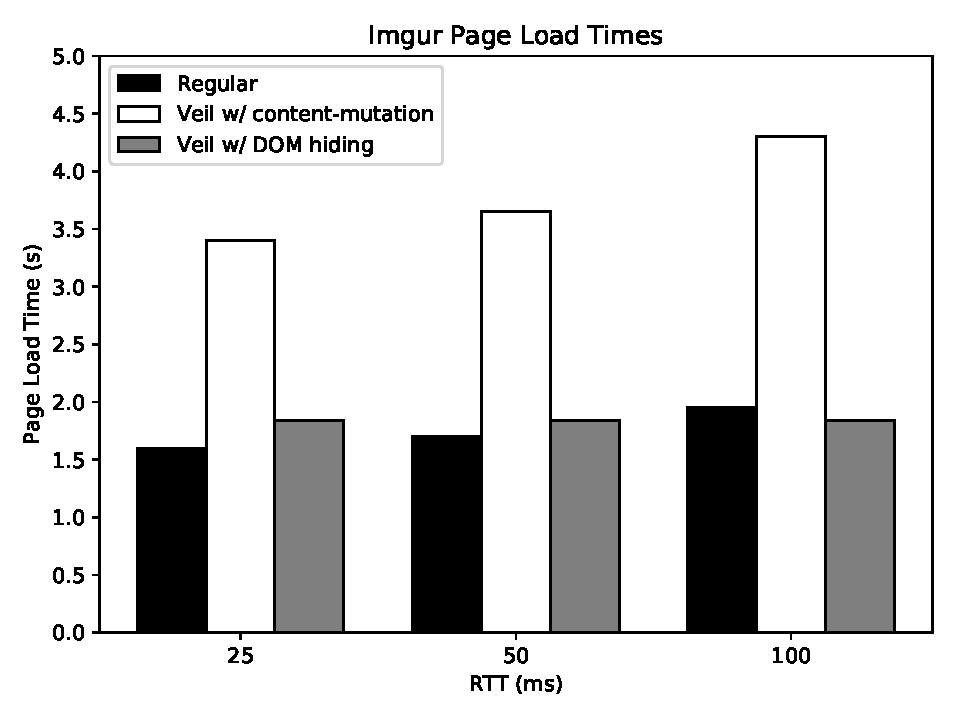
\includegraphics[width=\textwidth]{veil-figs/network_em.pdf}
	\caption[The impact of emulated network latency on page load
	times.]{The impact of emulated network latency on page load
		times. In all cases, the download bandwidth cap
		was 30 Mbps, and the upload bandwidth cap was 10
		Mbps, emulating a broadband connection. Bandwidth
		was not varied because page load times are largely
		governed by network latency, not bandwidth~\cite{gentleaggression}.}
	\label{fig:net_em}
\end{figure}

Figure~\ref{fig:net_em} uses Chrome's built-in network
emulation framework~\cite{chromeThrottle} to compare load times
for three versions of the Imgur page: a normal version;
a Veil version which used content mutation, heap
walking, and encrypted storage; and a Veil version
which used DOM hiding. The DOM hiding variant was largely
insensitive to increased network latency, since loading
a page only required two HTTP-level round trips (one to
fetch the bootstrap page, and another to fetch the initial
screenshot). The other variant of Veil was more sensitive
to network latency. The reason is that, in this version of
the page, the bootstrap code had to fetch multiple objects,
all of which were served from the same blinding server origin
(\texttt{https://veil.io}). Browsers cap the number
of simultaneous connections that a client can make to
a single origin, so the Veil page could not leverage
domain sharding~\cite{domainSharding} to circumvent the
cap. This limitation is not fundamental to Veil's design,
since content providers can shard across multiple blinding
server domains (e.g., \texttt{https://a.veil.io}
and \texttt{https://b.veil.io}). However (and
importantly), if a content provider wishes to use
sharding, the provider must be careful to avoid bias
in the mapping of objects to domains---otherwise,
per-site fingerprints may arise in a page's access
patterns to various domains. Thus, for some content
providers, domain sharding may not be worth the potential
loss in security.

Domain sharding is also relevant to Content Security
Policies (CSPs)~\cite{csp}. A CSP allows a page to restrict the
origins which can provide specific types of content.
For example, a CSP might state that a page can only
load JavaScript from \texttt{https://a.com}, and CSS
from \texttt{https://b.com}. A CSP is expressed as a
server-provided HTTP response header; the CSP is enforced
by the browser. CSPs are useful for preventing cross-site
scripting attacks, but require a page to be able to
explicitly shard content across domains. As discussed
in the last paragraph, Veil can enable sharding at
the cost of reduced security.

\subsection{Related Work}
\label{sec:related}

%{\bf Interactions with the Cloud}\\
%Mylar~\cite{mylar} is a platform for building
%secure web applications atop untrusted servers.
%Mylar only stores encrypted user data on servers,
%and decrypts that data using client-side JavaScript.
%Mylar defines primitives for searching over
%encrypted data and validating the JavaScript code
%that a potentially malicious server returns
%to the browser. Veil focuses on client-side
%privacy issues, but a Veil application could
%be layered atop Mylar to provide server-side
%protections as well.

%\
%{\bf Systems Support for Data Privacy:}
To minimize information leakage via RAM artifacts,
applications can use best practices like pinning
sensitive memory pages, and avoiding excessive
copying of secret data~\cite{harrison07}.
Operating systems and language runtimes can also
scrub deallocated memory as quickly as
possible~\cite{chow05}. Web browsers do not expose
low-level OS interfaces to JavaScript code, so
privacy-preserving sites cannot directly access
raw memory for the purposes of secure deallocation
or pinning. Determining the best way to expose
raw memory to JavaScript is an open research problem,
given the baroque nature of the same-origin policy,
and the fact that the browser itself may contend
with JavaScript code for exclusive access to a
memory page (e.g., to implement garbage collection
or tab discarding~\cite{tabDiscarding}).

An OS can protect RAM artifacts by encrypting
the swap space or the entire file system~\cite{blaze93,provos00,cryptfs}.
Veil's content mutation and DOM hiding allow Veil
to protect RAM artifacts even when a browser does not
run atop an encrypted storage layer. Content mutation
obviously does not provide a cryptographically strong
defense, but DOM hiding allows a Veil site to avoid
sending any site-specific, greppable content to a
client browser.

CleanOS~\cite{cleanOS} is a smartphone OS that
protects sensitive data when mobile devices
are lost or stolen. CleanOS defines sensitive
data objects (SDOs) as Java objects
and files that contain private user data.
CleanOS observes which SDOs are not actively
being used by an application, and encrypts
them; the key is then sent to the cloud, deleted
from the smartphone, and only retrieved when
the SDOs become active again. SDOs could
potentially be used as a building block for
private browsing. However, SDOs are insufficient
for implementing blinded references unless
the SDO abstraction is spread beyond the managed
runtime to the entire OS.

Lacuna~\cite{lacuna} implements private sessions
by running applications inside of VMs. Those VMs
execute atop the Lacuna hypervisor and a modified
Linux host kernel. The hypervisor and the host
kernel collectively implement ``ephemeral'' IO
channels. These encrypted channels allow VMs to
communicate with hardware or small pieces of
trusted code, but only the endpoints can access
raw data---user-mode host processes and the majority
of the host kernel can only see encrypted data.
Lacuna also encrypts swap memory. Upon VM
termination, Lacuna zeros the VM's RAM space and
discards the ephemeral session keys.
PrivExec~\cite{privExec} is similar to Lacuna,
but is implemented as an OS service instead of
a hypervisor.
%
% PrivExec~\cite{privExec} is an OS service that supplies
% privacy-seeking applications with automatically encrypted
% channels to persistent storage. Similar to Lacuna, PrivExec
% associates private processes with ephemeral keys that are
% used to transparently encrypt writes to the file system
% and page file. PrivExec also monitors IPCs to ensure that
% private session data is not leaked to non-private processes.
% Like Lacuna, PrivExec destroys ephemeral keys when applications
% terminate.
%
Lacuna and PrivExec provide stronger forensic
deniability than Veil. However, these systems
force layperson end-users to install and configure
a special runtime; furthermore, private applications
cannot persist data across sessions because keys are
ephemeral.

UCognito~\cite{ucognito} exposes a sandboxed file system
to a private browsing session. The sandboxed file system
resides atop the normal one, absorbing writes made during
private browsing. When the browsing session terminates,
UCognito discards the writes. Like PrivExec and Lacuna,
UCognito requires a modified client-side software stack.
UCognito also does not protect against information leakage
via the non-sandboxed parts of the host OS. For example,
unmodified RAM artifacts may page to the native swap file;
DNS requests are exposed to the host's name resolution
subsystem.

Amazon Silk~\cite{amazon-silk} is a browser used on Amazon
Kindles and uses a technique called remote dependency 
resolution (also known as split browsing)~\cite{rc2, parcel}. 
When the Silk client issues an HTTP request for a web page,
the request actually goes to an Amazon-maintained 
proxy that runs in the cloud. The proxy then uses a headless
browser to load the requested page. Since the proxy lives
in the core of the Internet, the proxy can fetch objects
over low-latency network paths. As the proxy fetches these
objects, they are streamed back to the user. This technique
allows Silk to avoid high last-mile latencies afflicting the path
between the client and Internet core. However, the client-side Silk browser
still loads regular DOM objects, like HTML, Javascript, CSS, etc.,
thus not implementing DOM hiding that exists in Veil. It also
does not protect RAM artifacts or provide content mutation.

Collaborative browsing frameworks~\cite{lowet09,jigsawCollab}
allow multiple users with different browsers to
simultaneously interact with a shared view of a web
page. Like these frameworks, Veil's DOM hiding mode
has to synchronize the GUI inputs and rendering activity
that belong to a canonical version of a page. However,
Veil only needs to support one remote viewer. More
importantly, Veil's DOM hiding mode only exposes the
client browser to generic JavaScript event handlers, as
well as a bitmap display; in contrast, prior collaborative
browsing frameworks replicate a site-specific, canonical
DOM tree on each client browser. Prior frameworks also
do not use blinding servers to hide information from
client-side, name-centric interfaces like the DNS
cache.

Silo~\cite{silo} and the framework of Jiang et
al~\cite{jiang14} use client-side bootstrap
pages which dynamically overwrite themselves
with new content. Silo uses this technique to
layer a delta-encoding protocol atop HTTP;
Jiang's system uses dynamic assembly as a crude
copy-protection mechanism, so that users who
right click and ``Save as'' a page will only
store the initial bootstrap HTML and not the
dynamically assembled content. By itself,
dynamic assembly cannot provide strong privacy
guarantees. For example, blinded URLs are needed
to prevent information leakage through the DNS
cache and the browser cache.

\subsection{Conclusions}
Veil is the first web framework that allows
developers to implement private-session semantics
for their pages. Using the Veil compiler,
developers rewrite pages so that all page content
is hosted by blinding servers. The blinding servers
provide name indirection, preventing sensitive
information from leaking to client-side, name-based
system interfaces. The blinding servers mutate
content, making object fingerprinting more
difficult; rewritten pages also automatically
encrypt client-side persistent storage, and
actively walk the heap to reduce the likelihood
that in-memory RAM artifacts will swap to disk in
cleartext form. In the extreme, Veil transforms
a page into a thin client which does not include
any page-specific, greppable RAM artifacts. Veil
automates much of the effort that is needed to
port a page to Veil, making it easier for
web developers to improve the privacy protections of
their applications.